\chapter{Część implementacyjna}

\section{Zbiór narzędzi}
Implementacja robudowanego projektu nie była by możliwa gdyby nie zbiór narzędzi które w znaczy sposób ułatwiły i przyspieszyły cały proces. 
\begin{itemize}[leftmargin=1cm]
    \item Trello -- opracowanie zadań do poszczególnych etapów;
    \item Adobe XD -- prototypowanie aplikacji;
    \item Visual Studio Code -- środowisko programistyczne;
    \item Java 11 + Spring Boot -- backend;
    \item MongoDB -- baza danych;
    \item Angular 12 -- frontend;
    \item GitHub -- repozytorium kodu.
\end{itemize}

\section{Trello -- deklaracja zadań}
Przed rozpoczęciem pracy nad danym etapem, deklarowane były zadania przy użyciu programu \textit{Trello}. W każdym z etapów, w szczególności implemetacyjnych, starannie były grupowane opracowywane funkcje. Następnie były one rozkładane na podzadania, które ostatecznie deklarowano w programie. Takie rozwiązanie pozwoliło na implementację funkcjonalności powiązanych ze sobą w tym samym etapie. Każdy z etapów trwał mniej więcej dwa tygodnie.
\begin{figure}[H]
    \centering
    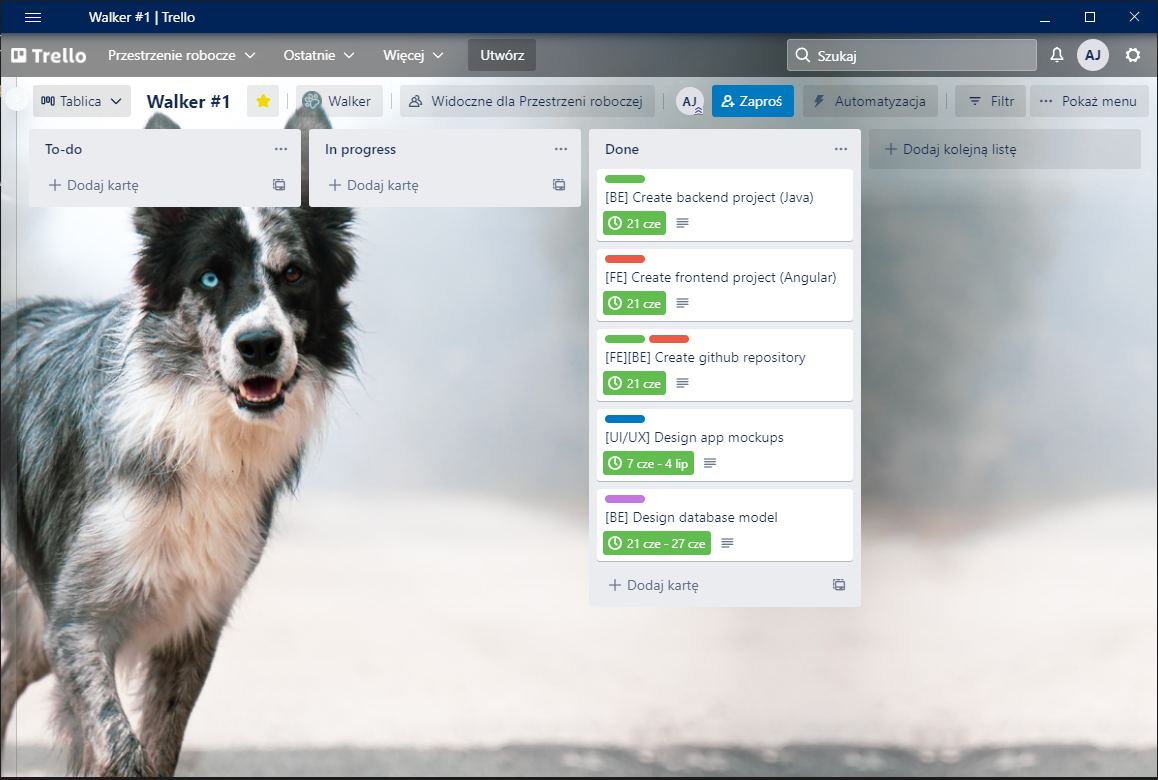
\includegraphics[width=1\linewidth]{rysunki/w1.PNG}
    \caption{Trello - tablica do pierwszego etapu}
    \label{fig:walker-board-1}
\end{figure}    

Do deklarowanych zadań dołączano odpowiedną etykietę, opis oraz listę podzadań, które były niezbędne przy danej funkcjonalności. Odpowiednie etykietowanie pozwoliło rozróżniać poszczególne zadania między sobą, a opis zawierał zaplanowane przez autora przypadki użycia danej funkcji.
Opisy etykiet:
\begin{itemize}[leftmargin=1cm]
    \item Zielony -- zadania dotyczące backendu;
    \item Czerwony -- zadania dotyczące frontendu;
    \item Niebieski -- zadania dotyczące projektu UI/UX aplikacji;
    \item Fioletowy -- zadania dotyczące bazy danych
    \item Żółty -- zadania oznaczone jako bugi, problemy w programie
\end{itemize}

Łącznie powstały cztery tablice, różniące się ilością oraz stopniem skomplikowania zadań.
\begin{enumerate}[leftmargin=1cm]
  \item \textbf{Walker \#1} -- etap pierwszy, skupiający się na inicjalizacji projektu, stworzenie prototypów aplikacji oraz zamodelowanie bazy danych;
  \item \textbf{Walker \#2} -- etap drugi, skupiający się na implementacji rejestracji oraz logowania użytkowników, oraz podstawowych komponentów aplikacji frontendowej między innymi pasek nawigacyjny, strona tytułowa, strona główna;
  \item \textbf{Walker \#3} -- etap trzeci, skupiający się na podstawowych funkcjonalnościach serwisu - tworzenie profilu psa, spaceru, pobieranie listy dostępnych spacerów, zapisywanie oraz wypisywanie się ze spaceru. Ponad to dodano możliwość edycji danych użytkownika;
  \item \textbf{Walker \#4} -- etap czwarty, skupiający się na implementacji oceny opiekunów oraz psów. Dodano również panel administracyjny do zarządzania aplikacją.
\end{enumerate}

\begin{figure}[H]
    \centering
    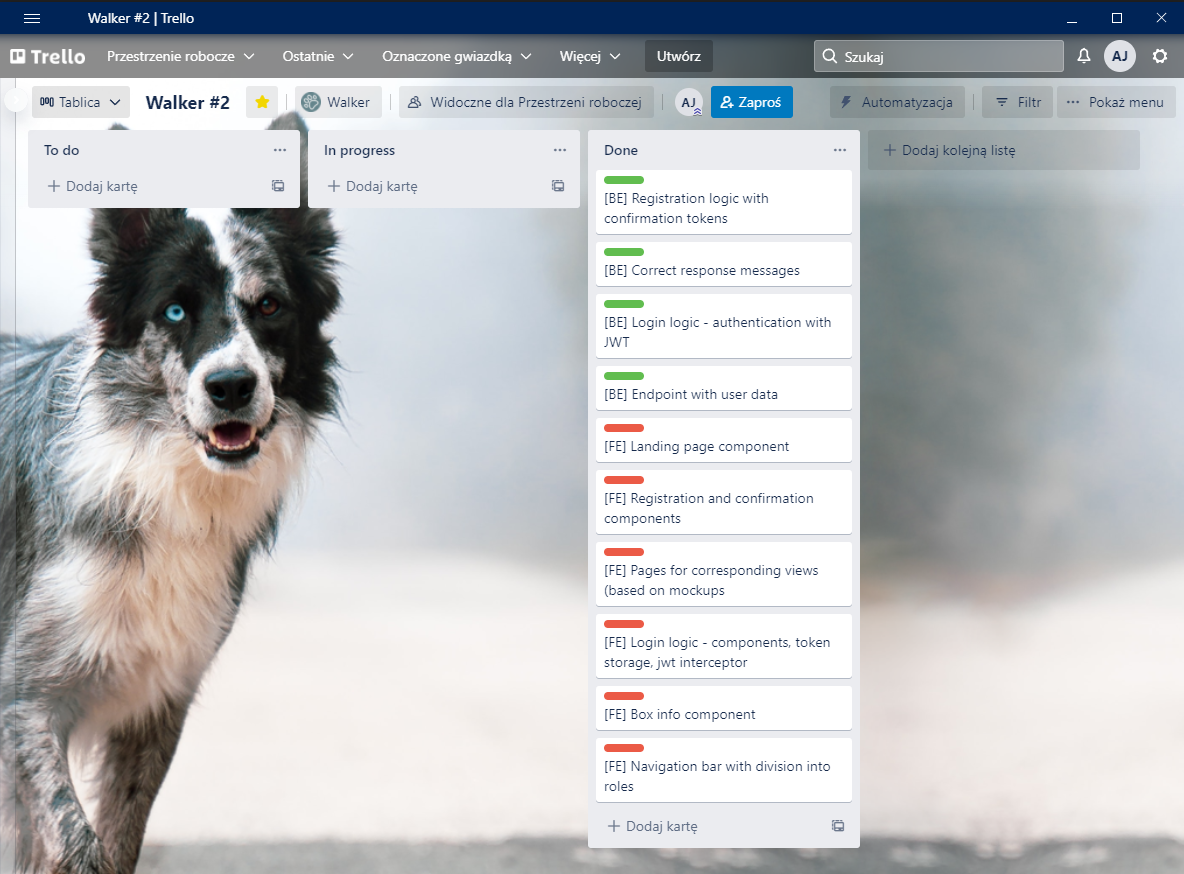
\includegraphics[width=1\linewidth]{rysunki/w2.PNG}
    \caption{Trello - tablica do drugiego etapu}
    \label{fig:walker-board-2}
\end{figure}  

\section{Adobe XD -- projektownaie prototypów}
Etap projektowania rozpoczęto od wyboru odpowiedniego zdjęcia przewodniego aplikacji, dobraniu palety kolorystycznej oraz stworzeniu logo serwisu. Zdjęcie przewodnie zostało znalezione na stronie z darmowymi zdjęciami. Na podstawie tego zdjęcia wygenerowano paletę kolorów, która została wykorzystana najpierw do prototypowania, a następnie już w samej aplikacji.
\begin{figure}[H]
    \centering
      \begin{tabular}{@{}ll@{}}
        
\includegraphics[width=0.475\textwidth]{rysunki/Start.png} & 
        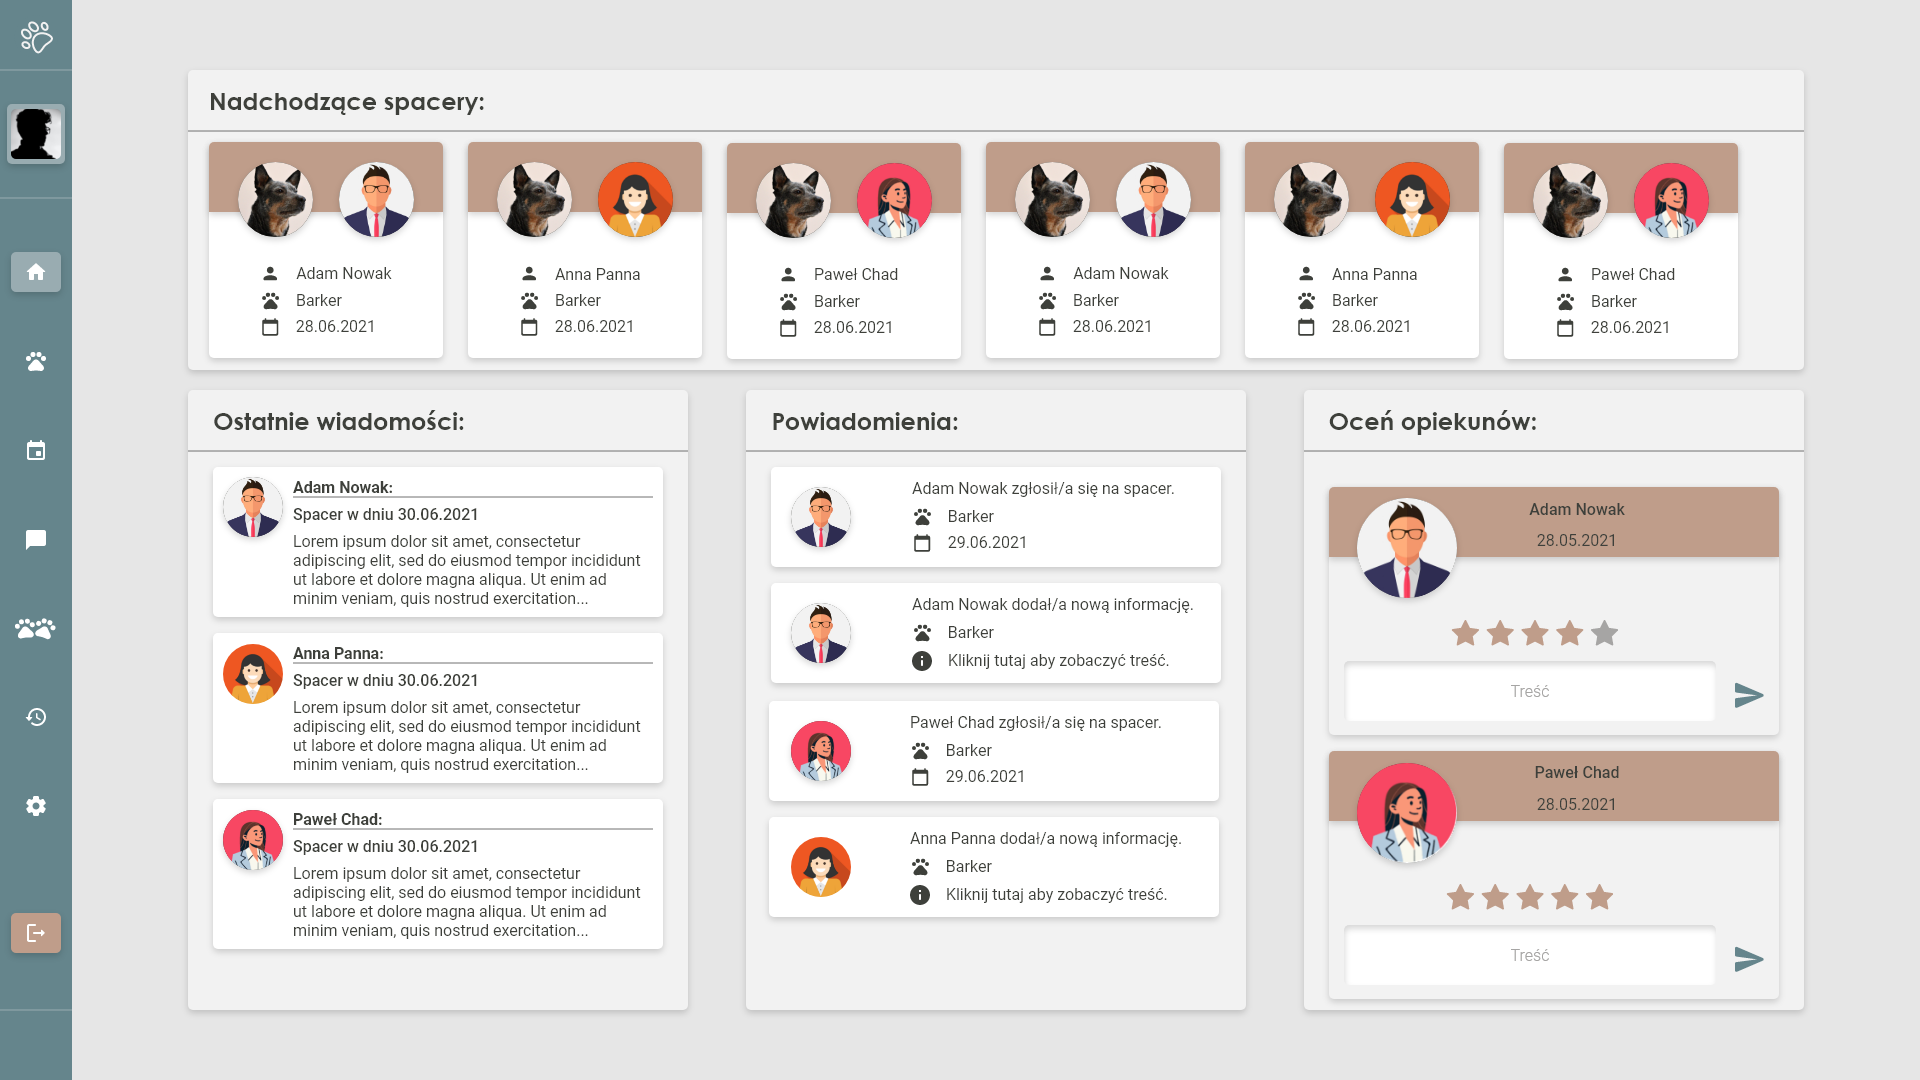
\includegraphics[width=0.475\textwidth]{rysunki/Home - owner.png}
      \end{tabular}
    \caption{Przykładowe prototypy aplikacji -- widok startowy, widok dashboardu}
    \label{fig:mocks-start-dashboard}
\end{figure}
\begin{figure}[H]
    \centering
      \begin{tabular}{@{}ll@{}}
        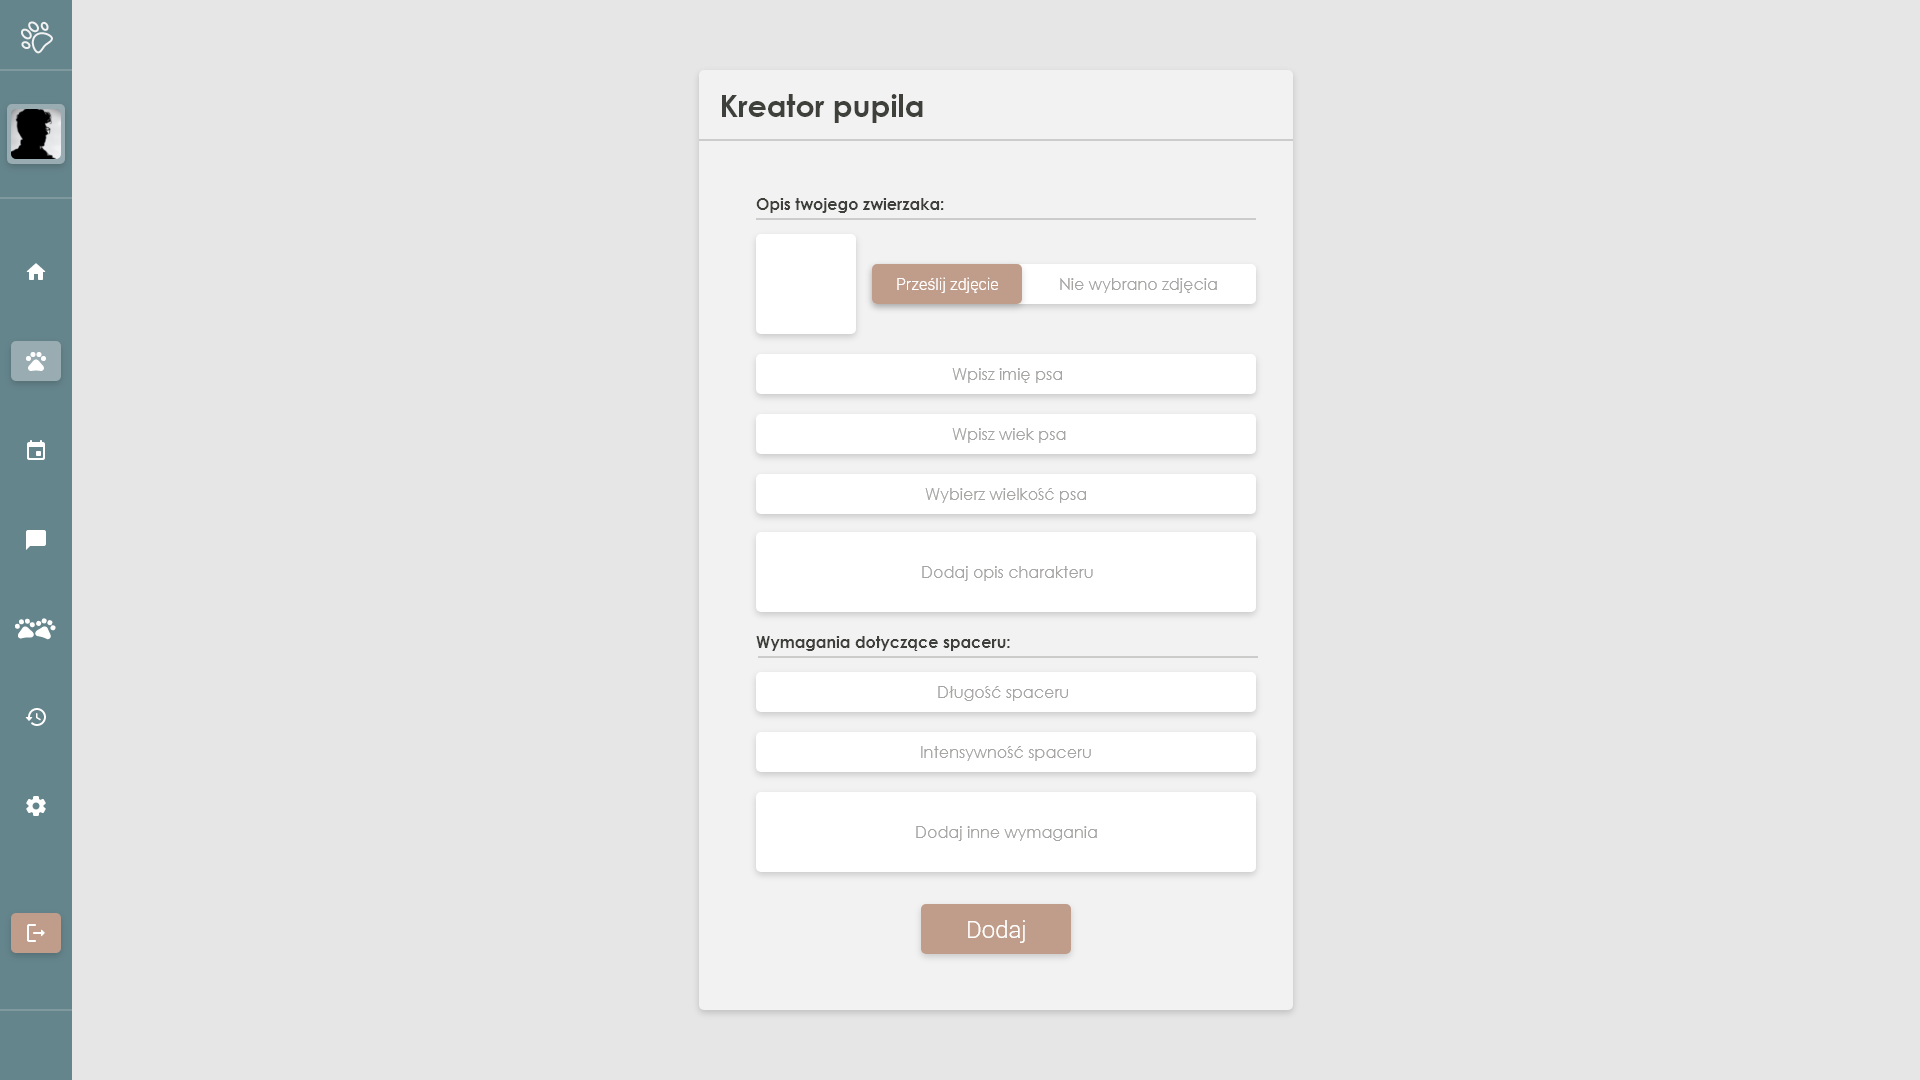
\includegraphics[width=0.475\textwidth]{rysunki/Home - dog creator.png} & 
        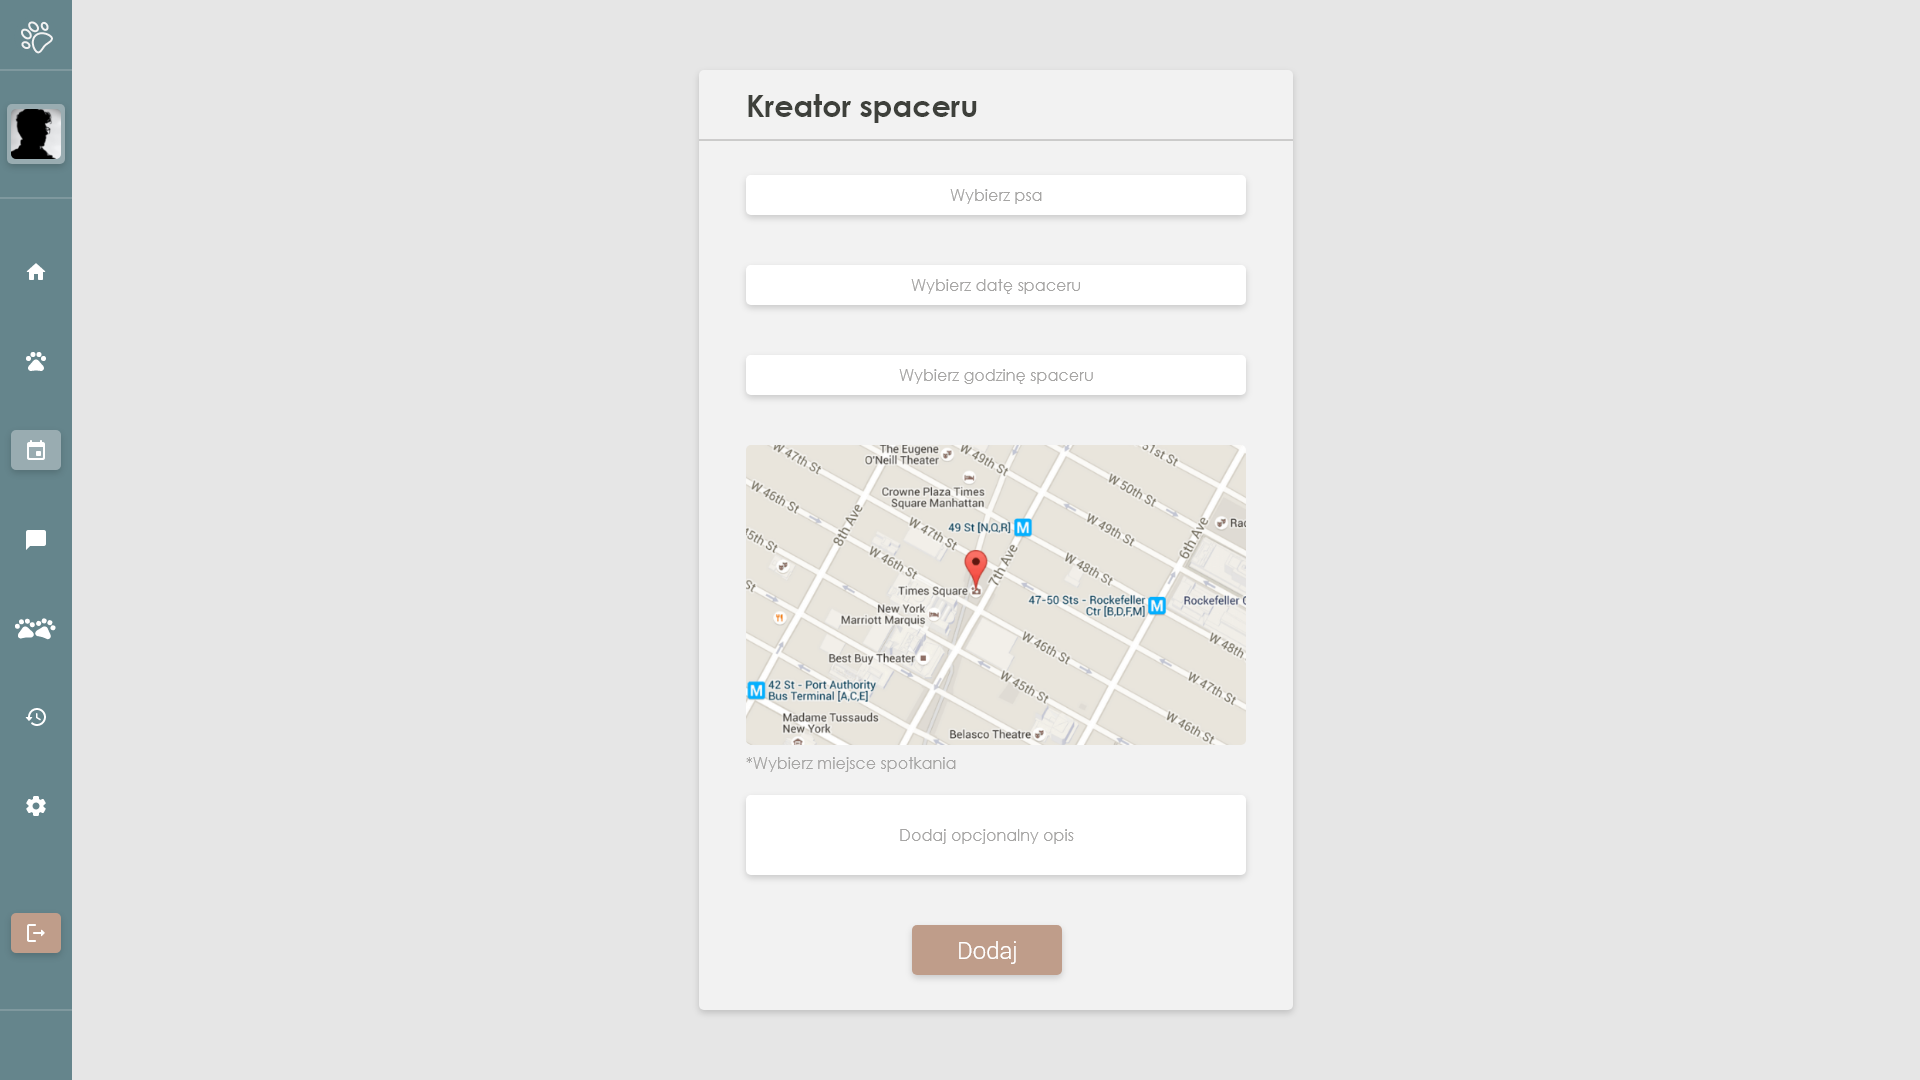
\includegraphics[width=0.475\textwidth]{rysunki/Home - walk creator.png}
      \end{tabular}
    \caption{Przykładowe prototypy aplikacji -- widok startowy, widok dashboardu}
    \label{fig:mocks-creators}
\end{figure}

Przy projektowaniu widoków posłużono się podstawowymi kształtami, głównie różnego rodzaju prostokątami oraz polami tekstowymi. Zastosowanie podstawowych właściwości tych elementów umożliwiło tworzenie atrakcyjnych komponentów, które były następnie rozmieszane na poszczególnych widokach. Cały proces miał na celu stworzenie makiet aplikacji, które cechowały by się atrakcyjnym wyglądem oraz umożliwiły by wizualizację założonych funkcjonalności. Na podstawie prototypów możliwe było również określenie maskymalnej długości znaków, które byłyby wyświetlane już w domyślnej aplikacji. Pozwoliło to na dostosowanie pól tekstowych tak, aby w dużym stopniu integrowały się z całym wyglądem aplikacji.
\begin{figure}[H]
    \centering
      \begin{tabular}{@{}ll@{}}
        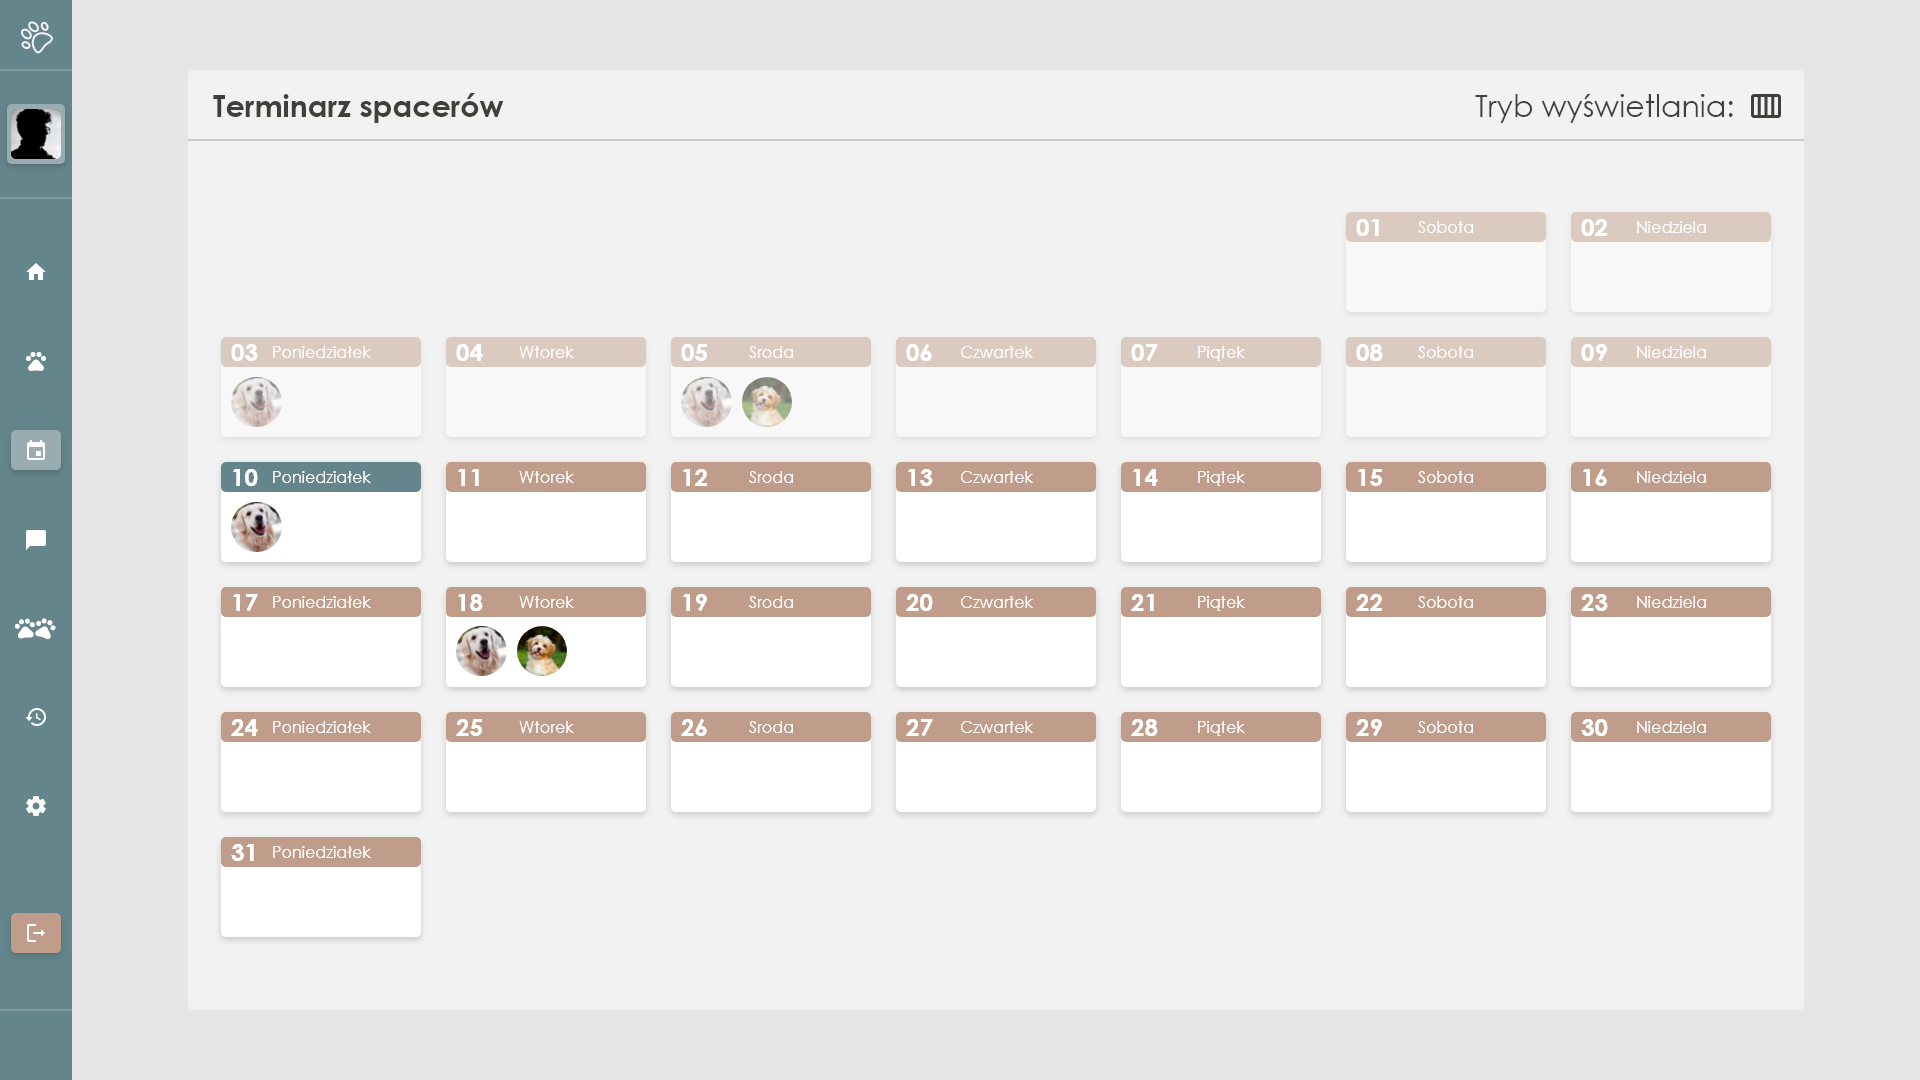
\includegraphics[width=0.475\textwidth]{rysunki/Home - walk calendar month.png} & 
        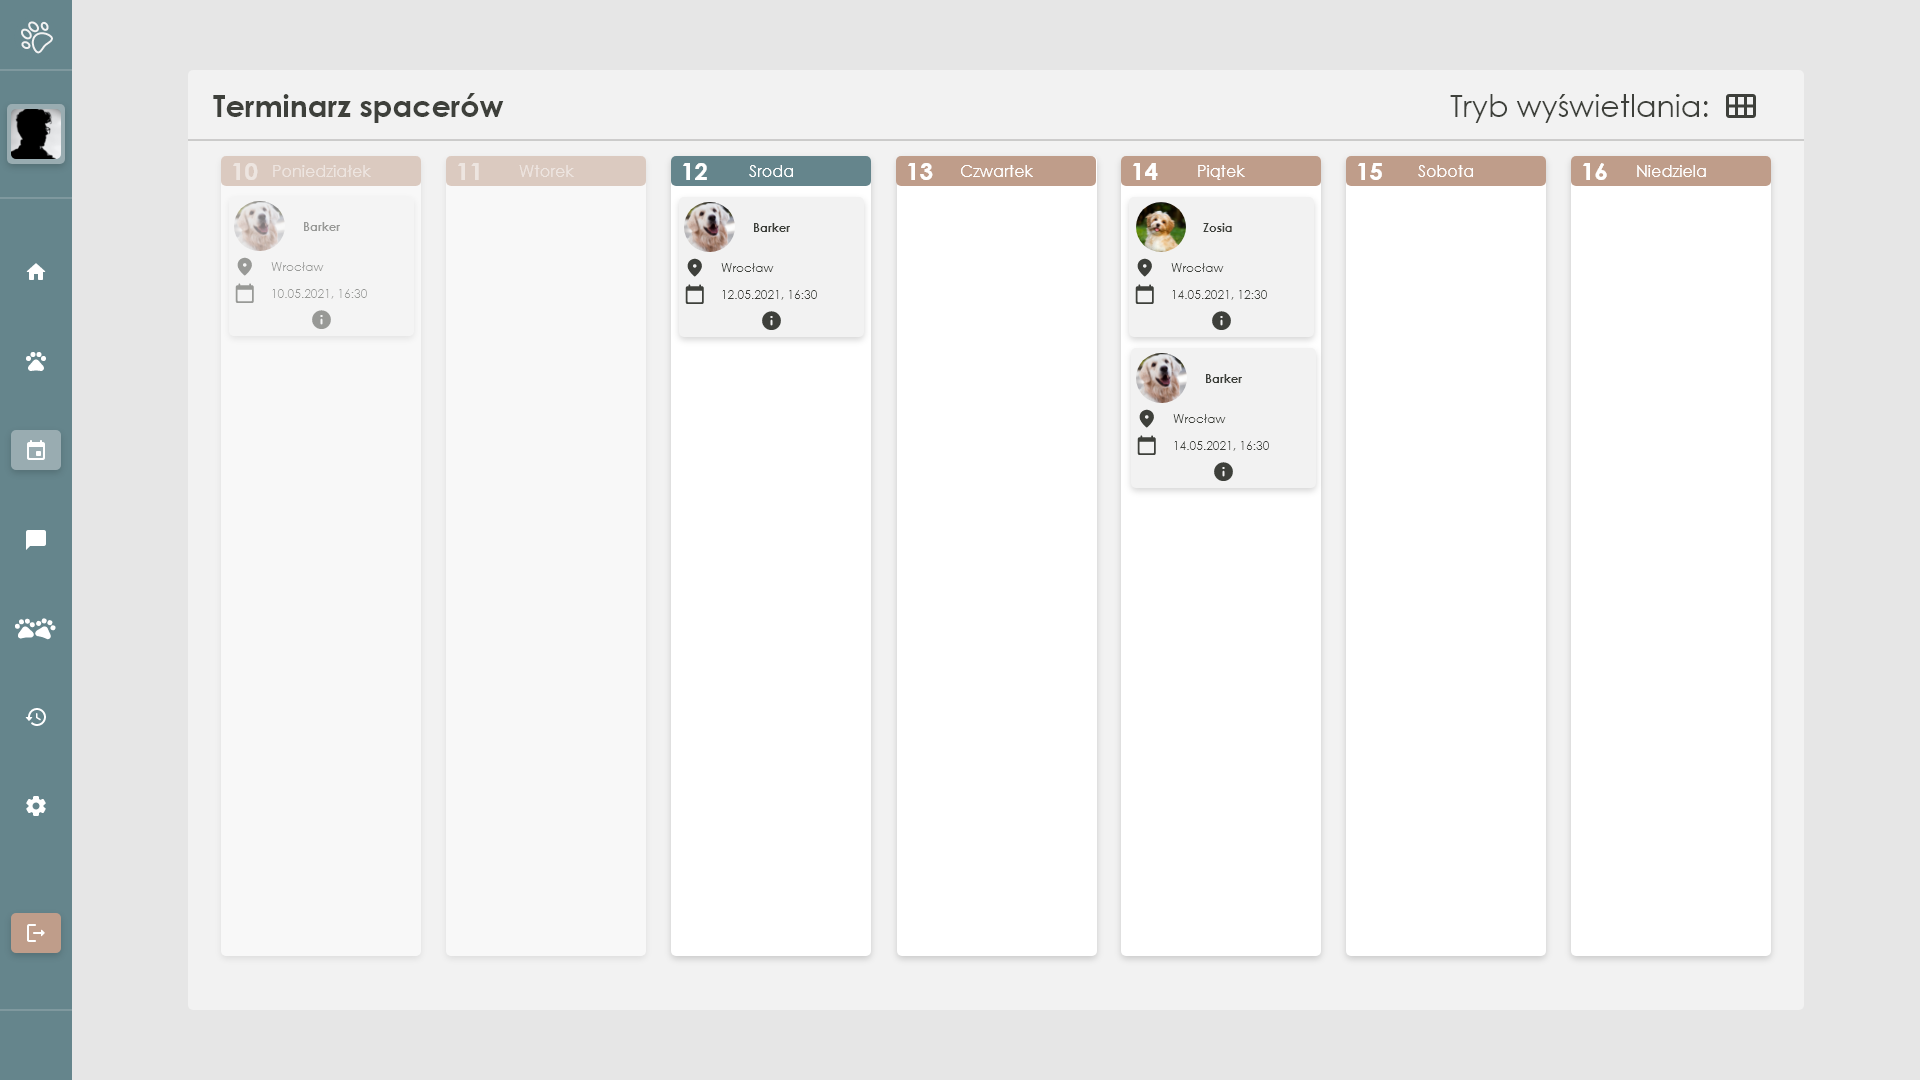
\includegraphics[width=0.475\textwidth]{rysunki/Home - walk calendar week.png}
      \end{tabular}
    \caption{Przykładowe prototypy aplikacji -- widok startowy, widok dashboardu}
    \label{fig:mocks-calendars}
\end{figure}
\begin{figure}[H]
    \centering
      \begin{tabular}{@{}ll@{}}
        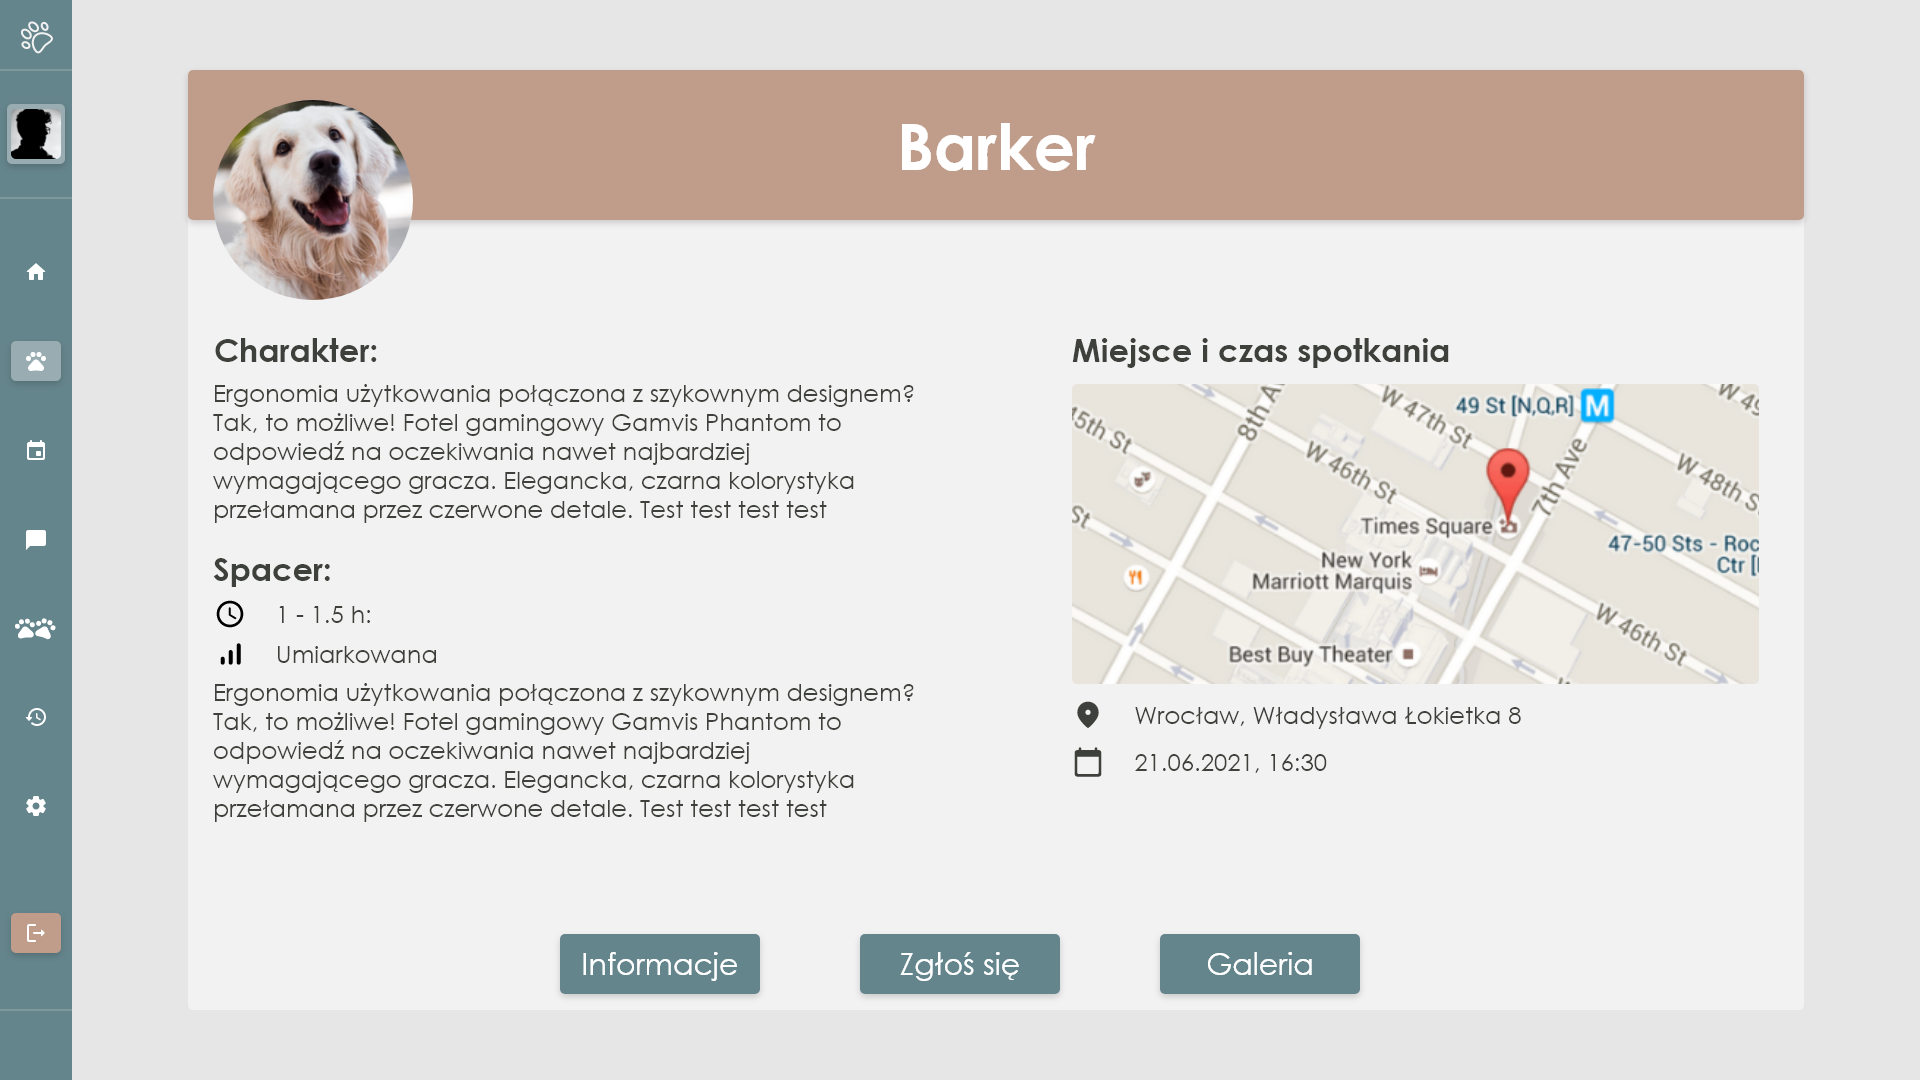
\includegraphics[width=0.475\textwidth]{rysunki/Home -walk info.png} & 
        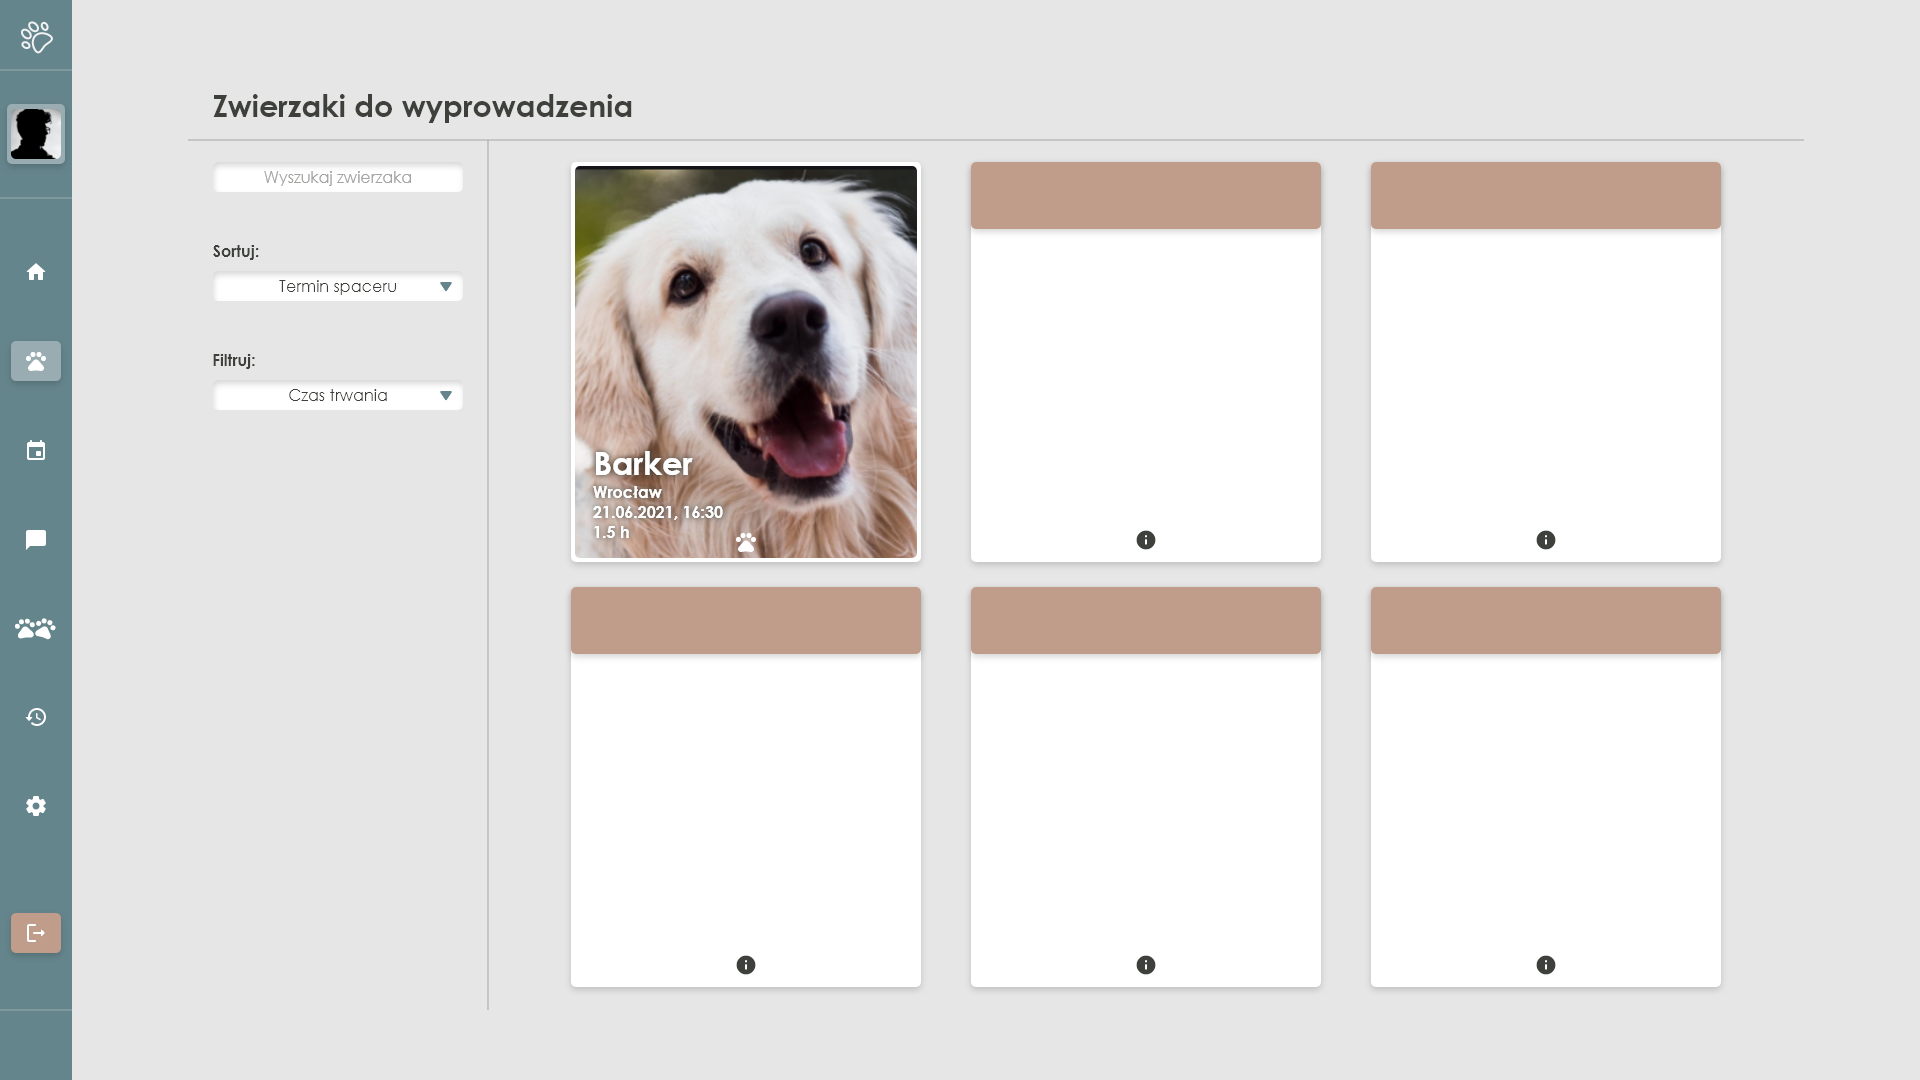
\includegraphics[width=0.475\textwidth]{rysunki/Home - dog list.png}
      \end{tabular}
    \caption{Przykładowe prototypy aplikacji -- widok startowy, widok dashboardu}
    \label{fig:mocks-lists}
\end{figure}

\newpage
\section{Java -- backend aplikacji}
Proces tworzenia warstwy logicznej rozpoczęło skonfigurowanie pliku \textit{application.properties}. Przechowuje on dane w postaci klucz - wartość, które służą między innymi do konfiguracji różnych składowych aplikacji np. połączenia z bazą danych lub konfiguracji przesyłanych plików. Można również deklarować dane, które można wykorzystać nastepnie w aplikacji. W taki sposób można zdefiniować globalne, stałe wartości, które można wykorzystać w trakcie pisania programu.
\begin{lstlisting}
spring.data.mongodb.database=walker
spring.data.mongodb.host=localhost
spring.data.mongodb.port=27017

jwtSecret=a43b97a5-4d2a-47bc-b74f-e677ebed35db
jwtExpiration=3600000

spring.servlet.multipart.max-file-size=10MB
spring.servlet.multipart.max-request-size=10MB
spring.servlet.multipart.enabled=true
\end{lstlisting}

\subsection{Architektura projektu}
Kolejnym, ważnym krokiem jest wykorzystanie odpowiedniej architektury projektu, pozwalającej na zachowanie porządku oraz grupowanie plików na postawie implementowanej logiki.

\begin{figure}[H]
  \centering
  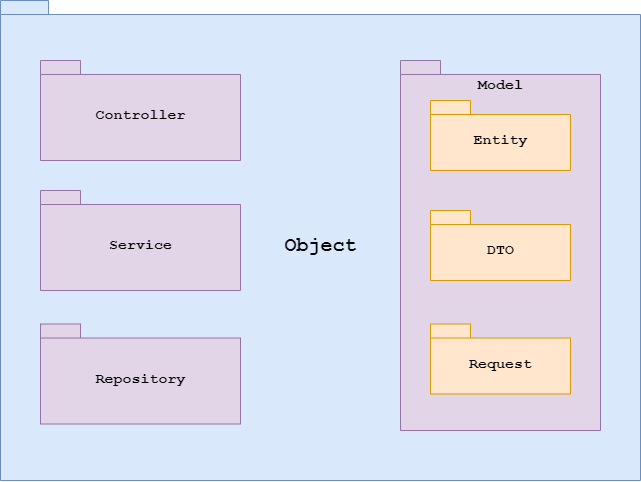
\includegraphics[width=1\linewidth]{rysunki/packages.png}
  \caption{Szczegółowa architektura - reprezentacja podfolderów}
  \label{fig:java-architecture-2}
\end{figure}

Postanowiono na podzielenie głównych folderów ze względu na konkretne obiekty.
W folderach głównych znajdują się podfoldery odpowiedzialne za przechowywanie: 
\begin{itemize}[leftmargin=1cm]
  \item \textit{Controller} -- przechowuje plik kontrolera, który udostępnia endpointy;
  \item \textit{Service} -- przechowuje plik serwisu, który posiada główną logikę związaną z danym obiektem;
  \item \textit{Repository} -- przechowuje plik repozytorium obiektu potrzebnego do komunikacji z bazą danych;
  \item \textit{Model}:
  \begin{itemize}
    \item \textit{Entity} -- obiekt rzutowany bezpośrednio na bazę danych;
    \item \textit{DTO} -- obiekt wysyłany do aplikacji dostępowej, bardziej rozbudowana encja o dodatkowe pola;
    \item \textit{Request} -- obiekt przesyłany bezpośrednio z aplikacji dostepowej po wypełnieniu formularzu;
  \end{itemize}
\end{itemize}

\begin{figure}[H]
  \centering
  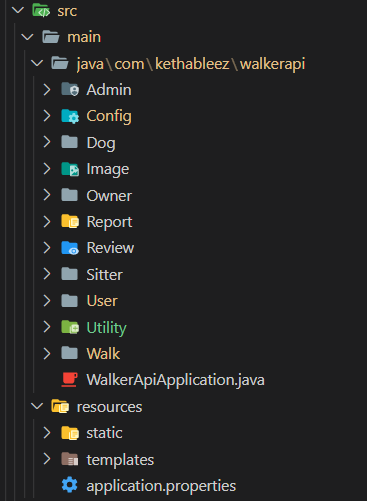
\includegraphics[width=0.5\linewidth]{rysunki/arch-java.PNG}
  \caption{Architektura projetku backendowego}
  \label{fig:java-architecture}
\end{figure}
Realna architura projektu zawiera dodatkowo folder konfiguracyjny. Znajdują się w nim pliki odpowiedzialne za konfigurację wykorzystanych zależności. Ponad to zdecydowano się na stworzenie folderu o nazwie \textit{Utility}, zawierającego narzędzia oraz funkcje wspomagające działanie aplikacji, na przykład funkcjonalność związaną z wyszukiwaniem spacerów po lokalizacji użytkownika.

\subsection{Zbiór oraz opis endpointów}
Punkty końcowe, znane w środowisku programistycznym też jako endpointy, wystawiane po stronie backendu służą do komunikacji z aplikacją dostępową poprzez protokół HTTP oraz jego metody. 
Do podstawowych metod można zaliczyć: 
\begin{itemize}[leftmargin=1cm]
  \item \textit{GET} -- pobieranie zasobu;
  \item \textit{POST} -- przesyłanie danych, często w ramach tworzenia nowego obiektu;
  \item \textit{PUT} -- przesyłanie danych, często w ramach edycji istniejącego już obiektu;
  \item \textit{DELETE} -- usuwanie zasobu.
\end{itemize}

\begin{figure}[H]
    \centering
    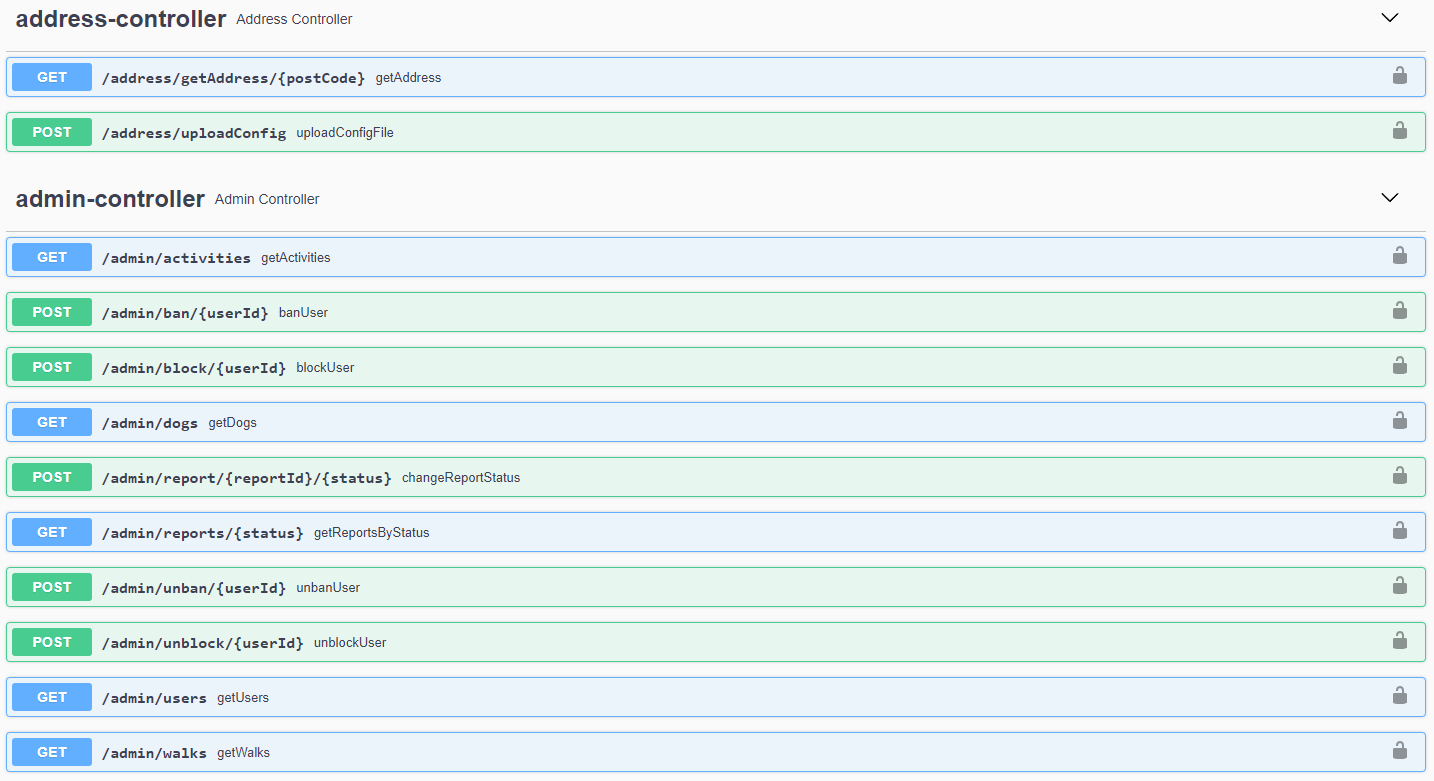
\includegraphics[width=1\linewidth]{rysunki/sw-1.PNG}
    \caption{Dokumentacja - AddressController, AdminController}
    \label{fig:swagger-1}
\end{figure}

\subsubsection{Address Controller}
Kontroler ten odpowiada za operacje związane z wyszukiwaniem adresu na podstawie kodu pocztowego. Ta funkcjonalność jest używana przy wyświetlaniu listy dostępnych spacerów na podstawie lokalizacji użytkownika, a dokładniej kodu pocztowego, który jest deklarowany przy rejestracji.
\begin{itemize}[leftmargin=1cm]
  \item \textit{uploadConfig} odpowiada za załadowanie pliku konfiguracyjnego, który jest odpowiednio przygotowanym plikiem, zawierającym zbiór województw, powiatów oraz ich unikalnych kodów. Taki plik jest przerabiany na encje, które następnie są ładowane do bazy danych. Pozwala to na wyszukiwanie odpowiedniej lokalizacji z poziomu backendu.
  \item \textit{getAddress} odpowiada za otrzymanie kodu związanego z powiatem na podstawie kodu pocztowego. Ta funkcjonalność opiera się o darmowe API Poczty Polskiej, pozwalające na otrzmanie odpowiedzi w formacie JSON z danymi o miejscowości po podaniu kodu pocztowego. 
\end{itemize}

\subsubsection{Admin Controller}
Udostępnia funkcje potrzebne na zarządzanie aplikacją przez administrację. Pozwala na blokowanie, banowanie oraz cofanie restrykcji na użytkownikach (endpointy: \textit{block, ban, unblock, unban}). Umożliwia pobieranie całej listy użytkowników, aktywności użytkowników, psów oraz spacerów z bazy danych. Dostarcza również metody związane z zarządzeniem zgłoszonymi błędami.

\begin{figure}[H]
    \centering
    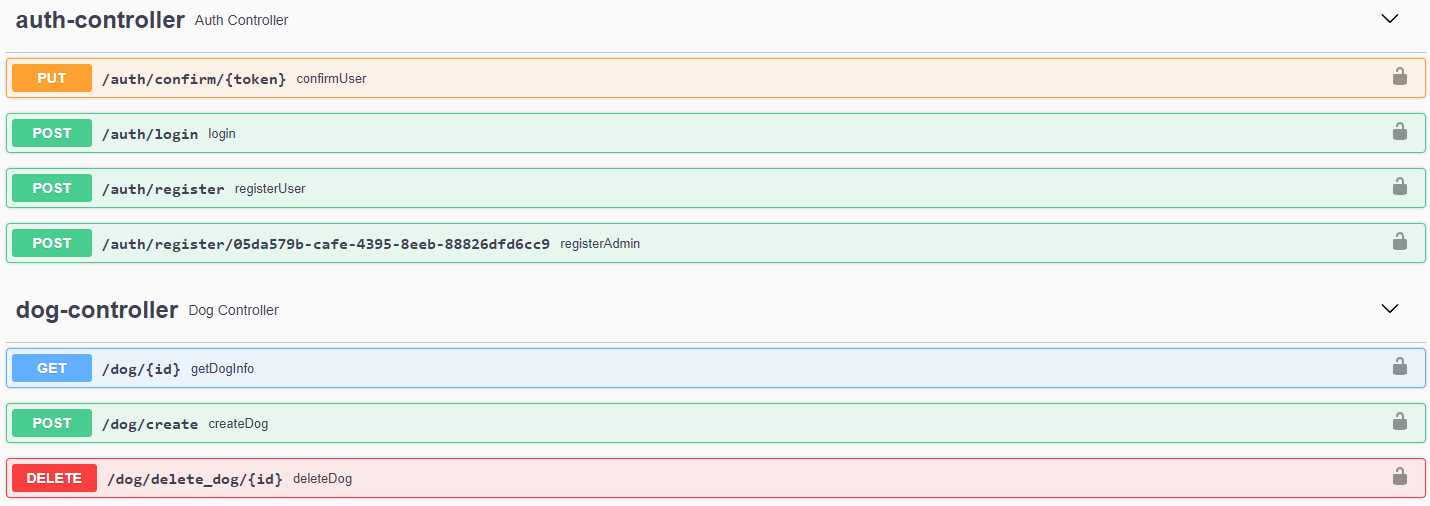
\includegraphics[width=1\linewidth]{rysunki/sw-2.PNG}
    \caption{Dokumentacja - AuthController, DogController}
    \label{fig:swagger-2}
\end{figure}
\subsubsection{Auth Controller}
Kontroler odpowiada za funkcjonalności związane z autoryzacją użytkowników. Pozwala na rejestrację oraz logowanie użytkowników. Szczegóły zostaly opiwane w podrozdziale \textit{3.4.3. JWT – Autoryzacja i autentykacja}. 

\subsubsection{Dog Controller}
Odpowiada za operacje związane z obiektem \textit{Dog}. Pozwala tworzyć nowy profil psa oraz pobierać szczegółowe informacje o danym zwierzaku po podaniu jego numeru ID.

\begin{figure}[H]
    \centering
    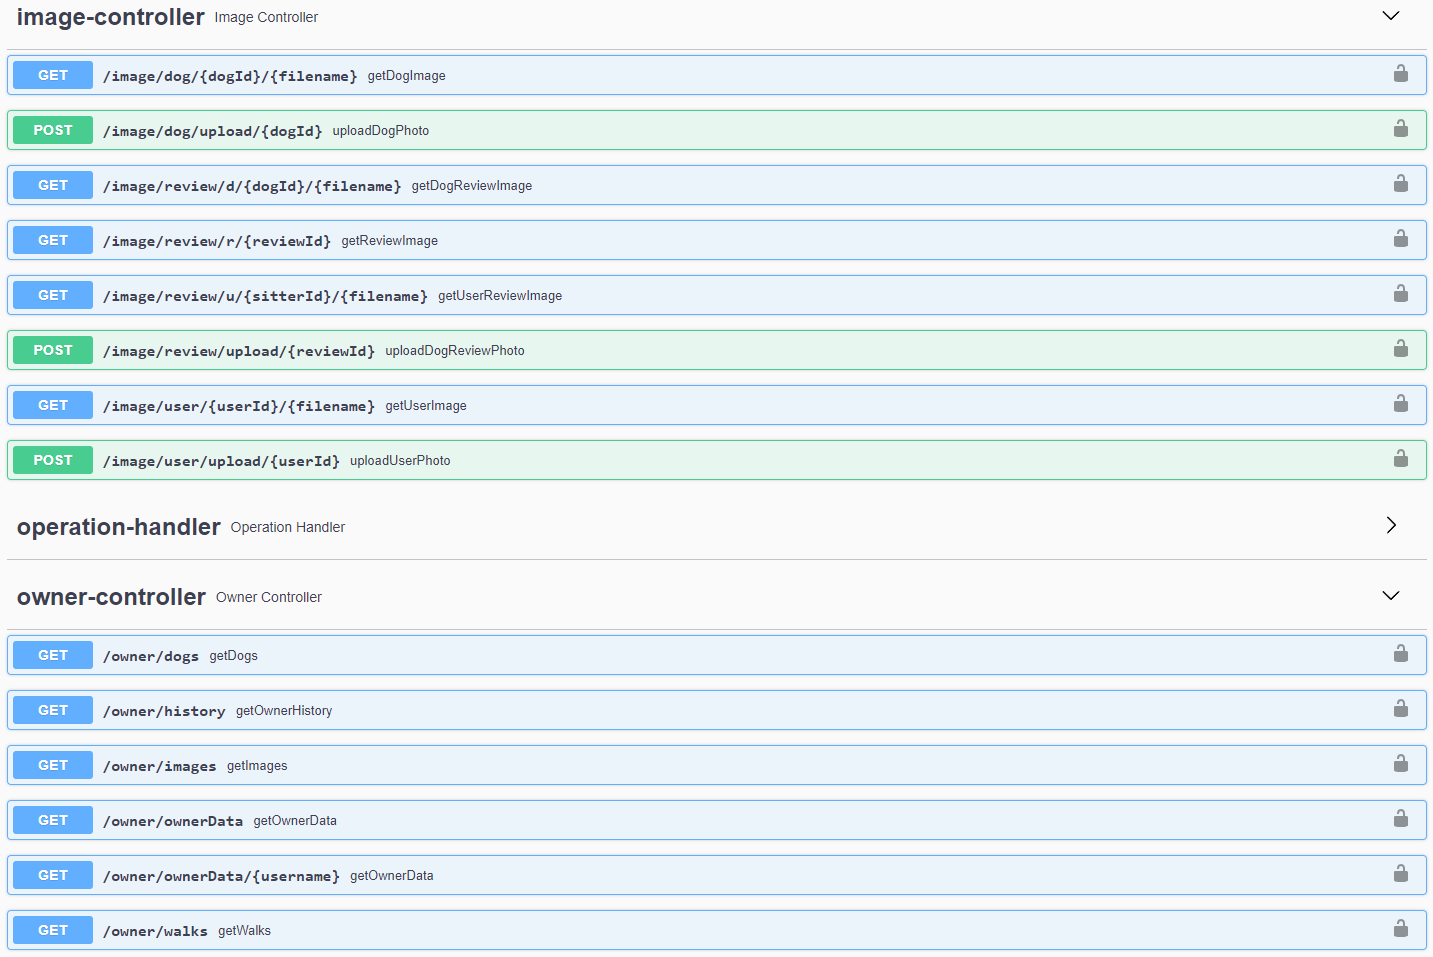
\includegraphics[width=1\linewidth]{rysunki/sw-3.PNG}
    \caption{Dokumentacja - ImageController, OwnerController}
    \label{fig:swagger-3}
\end{figure}
\subsubsection{Image Controller}
Udostępnia szereg endpointów pozwalających na zarządzanie zdjęciami. Umożliwia zapisywanie poszczególnych rodzajów zdjęci - użytkowników, psów oraz opinii, oraz otrzymywanie takich zdjęć z bazy danych.

\subsubsection{Owner Controller}
Kontroler odpowiada za wyświetlanie danych związanych z użytkownikami z rolą OWNER. Pozwala na wyświetlanie danych o właścicielu, jego historii, posiadanych psach oraz wszystkich zdjęć, które zostały dodane do jego psów.

\begin{figure}[H]
    \centering
    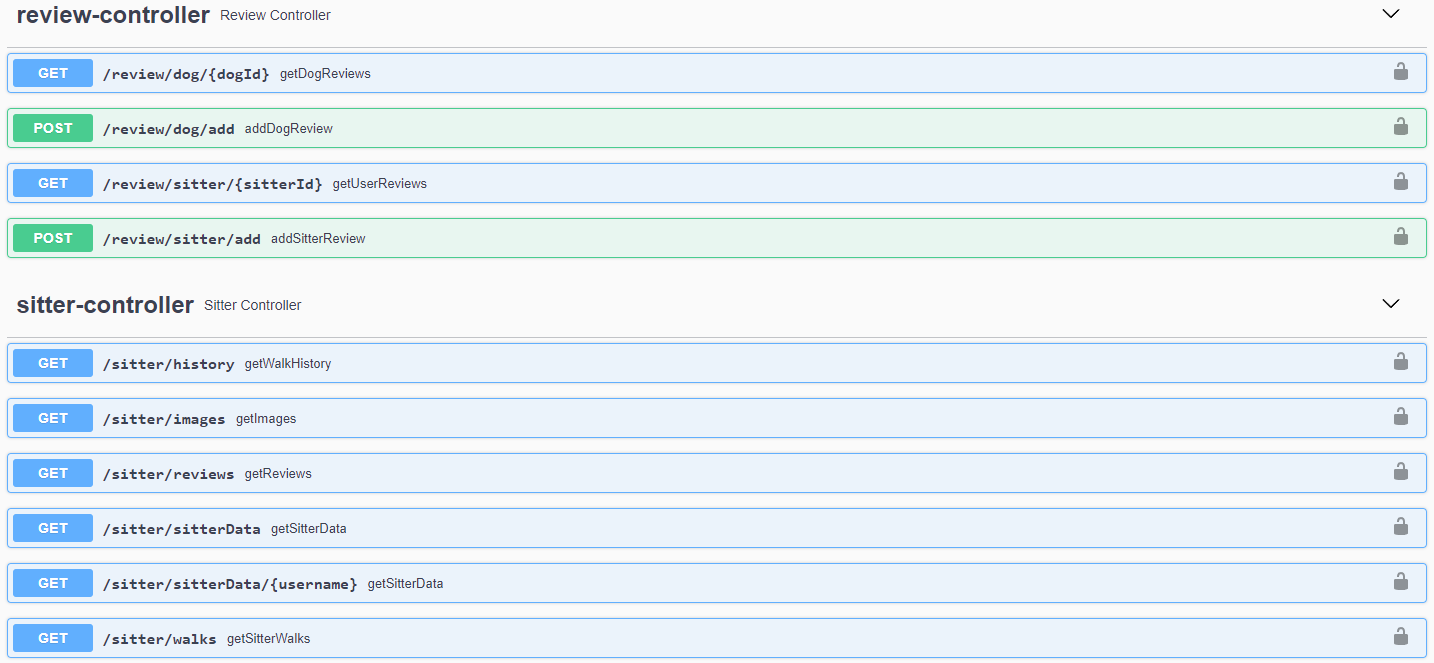
\includegraphics[width=1\linewidth]{rysunki/sw-4.PNG}
    \caption{Dokumentacja - ReviewController, SitterController}
    \label{fig:swagger-4}
\end{figure}
\subsubsection{Review Controller}
Udostępnia możliwość dodawania opinii do psów oraz opiekunów oraz pobieranie listy komentarzy.

\subsubsection{Sitter Controller}
Kontroler odpowiada za wyświetlanie danych związanych z użytkownikami z rolą SITTER. Pozwala na wyświetlanie danych o opiekunie, jego historii, opiniach dodanych przez innych użytkowników oraz wszystkich dostępnych zdjęciach.

\begin{figure}[H]
    \centering
    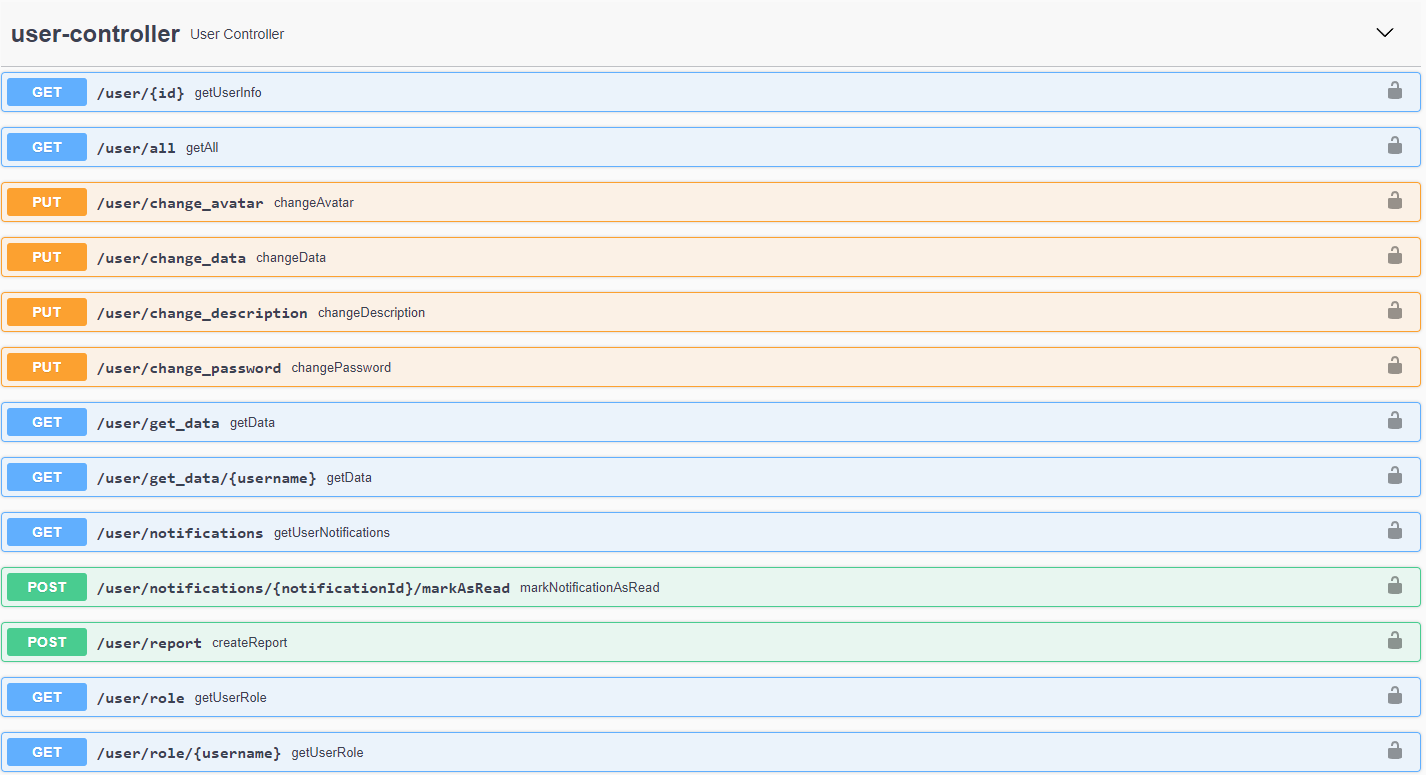
\includegraphics[width=1\linewidth]{rysunki/sw-5.PNG}
    \caption{Dokumentacja - UserController}
    \label{fig:swagger-5}
\end{figure}
\subsubsection{User Controller}
Pozwala na edycję danych użytkownika oraz pobieranie niezbędnych do działania aplikacji, informacjach. 

\begin{figure}[H]
    \centering
    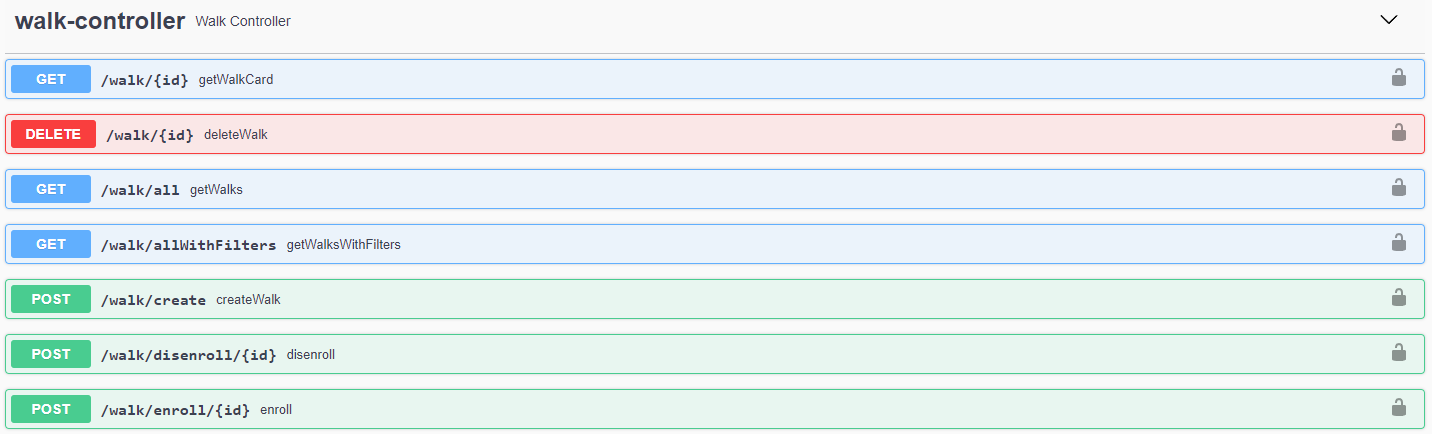
\includegraphics[width=1\linewidth]{rysunki/sw-6.PNG}
    \caption{Dokumentacja - WalkController}
    \label{fig:swagger-6}
\end{figure}
\subsubsection{Walk Controller}
Kontroler odpowiedzialny za tworzenie nowych spacerów, pobieranie listy dostępnych spacerów, zapisywanie oraz wyspisywanie się ze spacerów.

\subsection{JWT -- Autoryzacja i autentykacja}
Autoryzacja użytkowników jest obecnie często używanym mechanizmem. Pozwala na nadawanie użytkownikom odpowiednich ról, zabezpieczaniem enpoint
ów oraz kontrolerów aplikacji backendowej przed dostępem dla osób niepowołanych. Umożliwia również zabezpieczanie kont użytkowników poprzez zastosowanie enkrypcji haseł odpowiednim algorytmem, który jest dostępny od razu po dołączeniu do projektu zależności \textit{Spring Security}.
\begin{figure}[H]
  \centering
  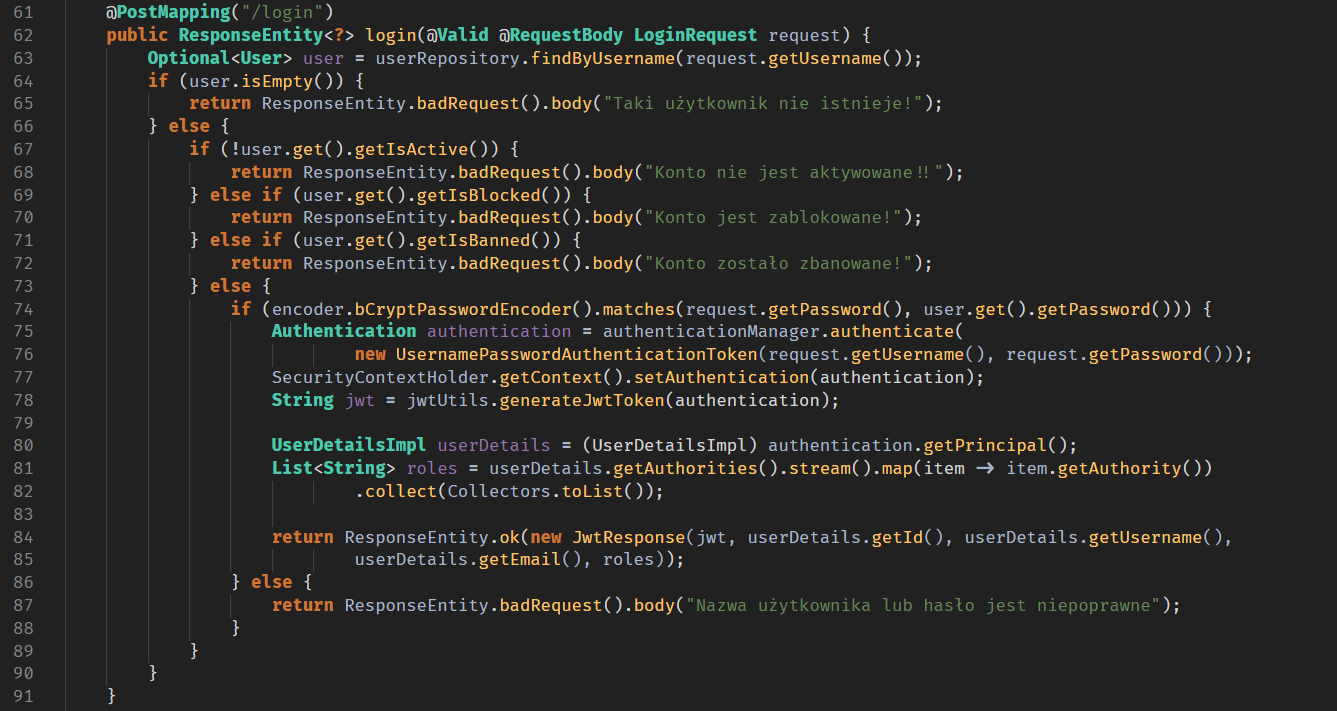
\includegraphics[width=1\linewidth]{rysunki/login.PNG}
  \caption{Implementacja logowania przy pomocy JWT}
  \label{fig:JWT}
\end{figure}  

Proces implementacji rozpoczęto od zamodelowania klasy użytkownika z odpowiednimi polami oraz stworzeniem ról użytkowników. Następnie dodano w klasie serwisowej logikę odpodziewzialną za dodawanie do użytkowniów ról oraz zapisywanie takich obiektów w bazie danych.

Kolejnym etapem była implementacja logiki związanej z JWT oraz logowaniem użytkowników. Proces logowania prezentuje się w nastepujący sposób:
\begin{itemize}[leftmargin=1cm]
  \item Przesłanie formularzu logowania z danymi -- nazwą użytkownika oraz hasłem;
  \item Sprawdzenie czy taki użytkownik znajduje się w bazie danych;
  \item Sprawdzenie, czy hasło odpowiada temu, które jest zapisane i zenkryptowane odpowiednim alogrytmem;
  \item W przypadku sukcesu, generowany jest token, zawierający dane: id, nazwę, email oraz role użytkownika;
  \item W przypadku niepowodzenia, do klienta wysyłany jest odpowiedni komunikat o błędzie.
\end{itemize}

\subsection{Implementacja wyszukiwania po lokalizacji}
Podczas tworzenia spaceru bądź rejestracji użytkownika, na podstawie kodu pocztowego podanego w formularzu, wysyłane jest zapytanie do API Poczty Polskiej o informacje związane z miejscowością, województwem oraz powiatem. Na podstawie tej odpowiedzi, w bazie danych wyszukiwany jest odpowiedni region i zwracane są kody -- powiatu oraz województwa. Kody następnie są dodawane do tworzonego obiektu.

\begin{figure}[H]
  \centering
  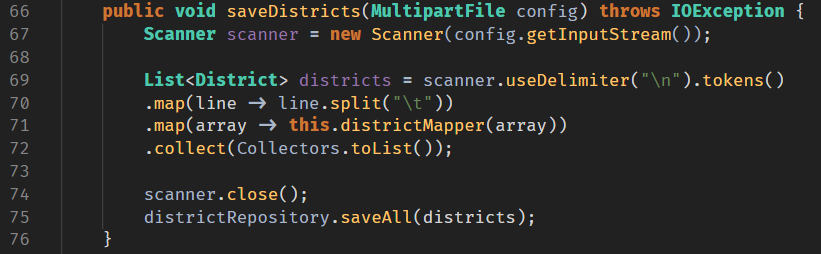
\includegraphics[width=1\linewidth]{rysunki/save.PNG}
  \caption{Implementacja zapisywania pliku konfiguracyjnego}
  \label{fig:config-file-implementation}
\end{figure}

Podczas wysyłania zapytania o listę dostępnych spacerów, po stronie backendu odbywa się filtrowanie listy wszystkich dostepnych spacerów. Pierwszym etapem jest pobranie informacji o regionie użytkownika, który wysłał zapytanie, następnie następuje filtrowanie spacerów po kodzie powiatu. W przypadku uzyskania pustej listy, następuje dodatkowe filtrowanie po kodzie województwa. Taka lista ostatecznie przesyłana jest do aplikacji dostępowej w celu jej prezentacji użytkownikowi.
\begin{figure}[H]
  \centering
  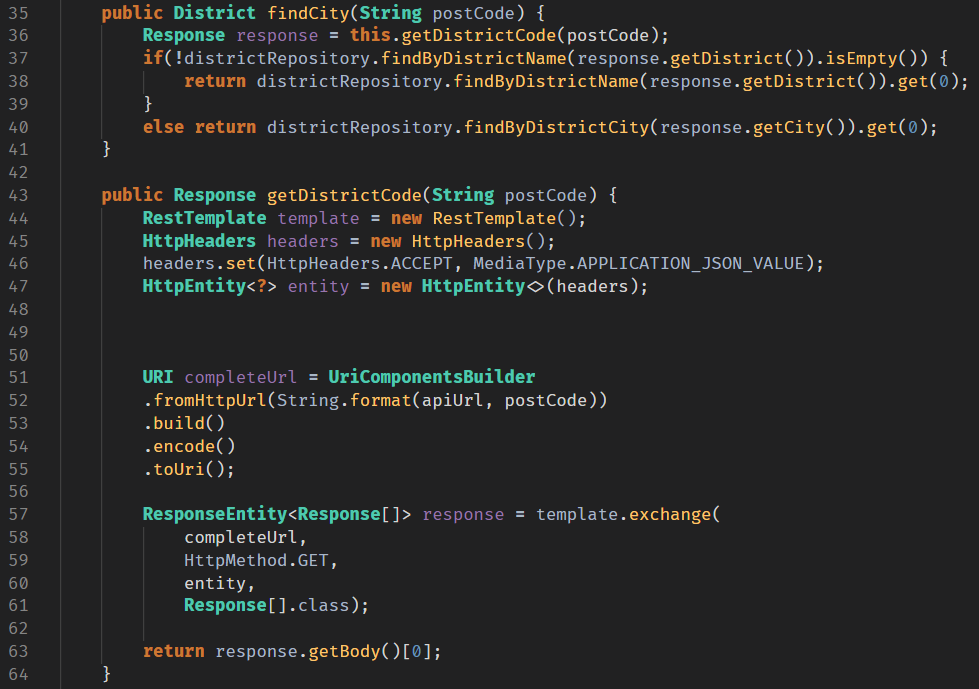
\includegraphics[width=1\linewidth]{rysunki/get-dist.PNG}
  \caption{Lista metod odpowiedzialnych za sprawdzanie lokalizacji}
  \label{fig:address-imlpementation}
\end{figure}

\subsection{Encje}
Nierelacyjne bazy danych charakteryzują się brakiem relacji między obiektami. Dlatego też, żeby połączyć odpowiadające obiekty w bazie, dodano do odpowiednich obiektów pola reprezentujące id powiązanych obiektów. Pozwoliło to na zachowanie porządku i spójności danych.
\begin{figure}[H]
  \centering
  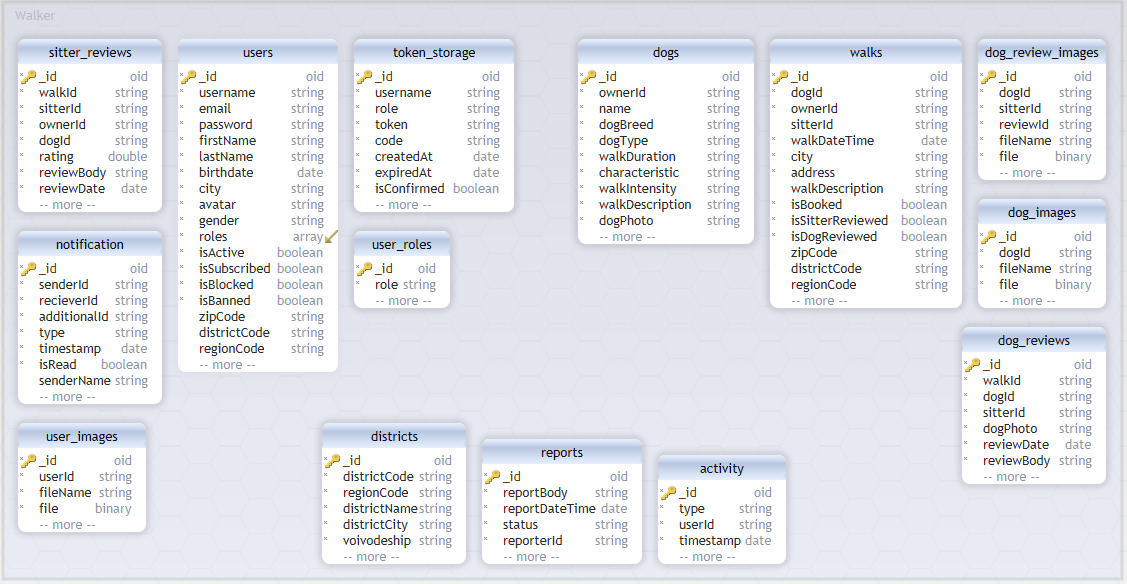
\includegraphics[width=1\linewidth]{rysunki/database.PNG}
  \caption{Widok bazy danych -- zbiór obiektów}
  \label{fig:database}
\end{figure}  
Obiekty, które są wysyłane do aplikacji dostępowej są złożonymi z kilku encji obiektami. Do tego użytko funkcji mapujących po stronie backendu. Takie funkcje mają za zadanie łączyć wiele obiektów ze sobą na podstawie wyżej wymienionego, dodatkowego pola id powiązanego obiektu.

\newpage
\section{Angular -- frontend}

\subsection{Konfiguracja projektu}
Proces konfiguracji rozpoczęło przystosowanie pliku \textit{environment.ts}.
\begin{lstlisting}
  export const environment = {
  apiBaseUrl: 'http://localhost:8080',
  urls,
};
\end{lstlisting}
\begin{itemize}
  \item apliBaseUrl -- deklaracja adresu URL, pod którym znajduje się backend aplikacji;
  \item urls -- zbiór dostępnych endpointów, pod które można wysyłać zapytanie.
\end{itemize}
Obiekt \textit{urls} jest zdefiniowany w następujący sposób:
\begin{lstlisting}
  ControllerName: {
    prefix: prefixName,
    calls: {
      endpoint: endpointName,
    },
  }
\end{lstlisting}
Takie rozwiązanie pozwoliło na deklarację wszystkich niezbędnych endpointów w jednym pliku konfiguracyjnym. Na potrzeby tego rozwiązania został stworzony plik serwisowy, który udostępnia szereg metod odpowiedzialnych za pobieranie, parsowanie oraz zwracanie odpowiednio spreparowanego adresu URL.

\begin{lstlisting}
  public getAuthUrl(action: string, params?: any) {
    return this.getUrl('auth', action, params);
  }
\end{lstlisting}
Wywołanie przykładowej metody rozpoczyna przekazanie do niej parametru \textit{action}, który określa pod jaki konkretnie endpoint będzie szło zapytanie oraz opcjonalny parametr \textit{params}, czyli zbiór parametrów wstrzykiwanych do adresu. Tak spreparowny adres jest przekazywany do metody odpowiedzialnej za wywoływanie zapytań oraz odbieranie odpowiedzi ze strony aplikacji backnedowej.

\subsection{Architektura projektu frontendowego}
Charakterystyka plików tworzonych w aplikacji frontendowej nie pozwala na zastosowanie omawianej wcześniej architektury użytej przy projekcie backendowym.
\begin{figure}[H]
  \centering
  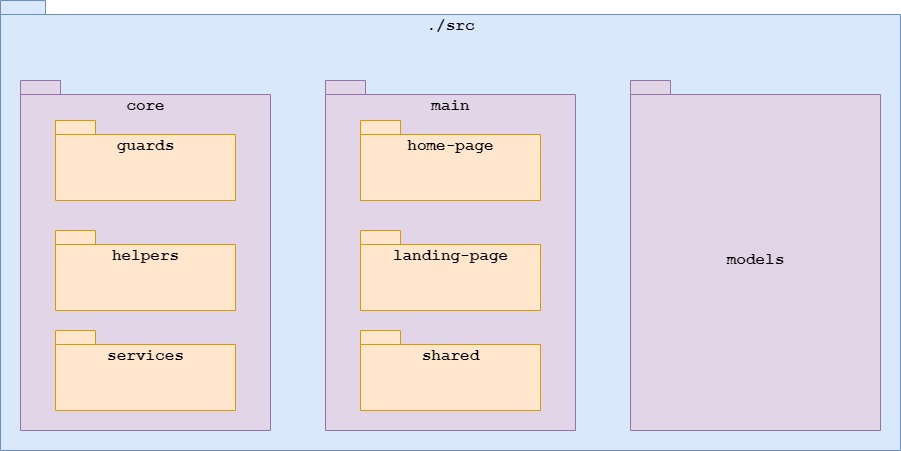
\includegraphics[width=1\linewidth]{rysunki/angular-arch.png}
  \caption{Architektura -- reprezentacja graficzna}
  \label{fig:angular-architecture}
\end{figure}
Podział został uwarunkowany przeznaczeniem plików. Architektura prezentuje się zatem następująco:
\begin{itemize}[leftmargin=1cm]
  \item \textbf{core} -- przechowuje podstawowe funkcjonalności:
  \begin{itemize}
    \item \textbf{guards} -- zawiera implementację klasy, która na podstawie roli użytkownika, pozwala lub wzbrania na dostęp do poszczególnych widoków aplikacji;
    \item \textbf{helpers} -- zawiera implementację klasy, odpowiedzialnej za wstrzykiwanie do każdego wysyłanego zapytania token autoryzacyjny zalogowanego użytkownika;
    \item \textbf{services} -- zawiera wszystkie serwisy, które są używane w aplikacji.
  \end{itemize}
  \item \textbf{main} -- przechowuje główne widoki oraz komponenty z wyróżnieniem na dwa główne widoki: stronę domową oraz stronę startową aplikacji:
  \begin{itemize}
    \item \textbf{home-page} -- zawiera implementację widoków, komponentów z rozróżnieniem na role użytkowników;
    \item \textbf{landing-page} -- przechowuje komponenty wykorzystywane przy stronie startowej takie, jak formularze logowania, rejestracji;
    \item \textbf{shared} -- w tym folderze zawarte są implementacje komponentów, które są wykorzystywane w każdym miejscu w aplikacji na przykład komponent odpowiedzialny za wyświetlanie komunikatów;
  \end{itemize}
  \item \textbf{models} -- przechowuje modele obiektów używanych w aplikacji.
\end{itemize}

\subsection{Działanie}
\begin{figure}[H]
  \centering
  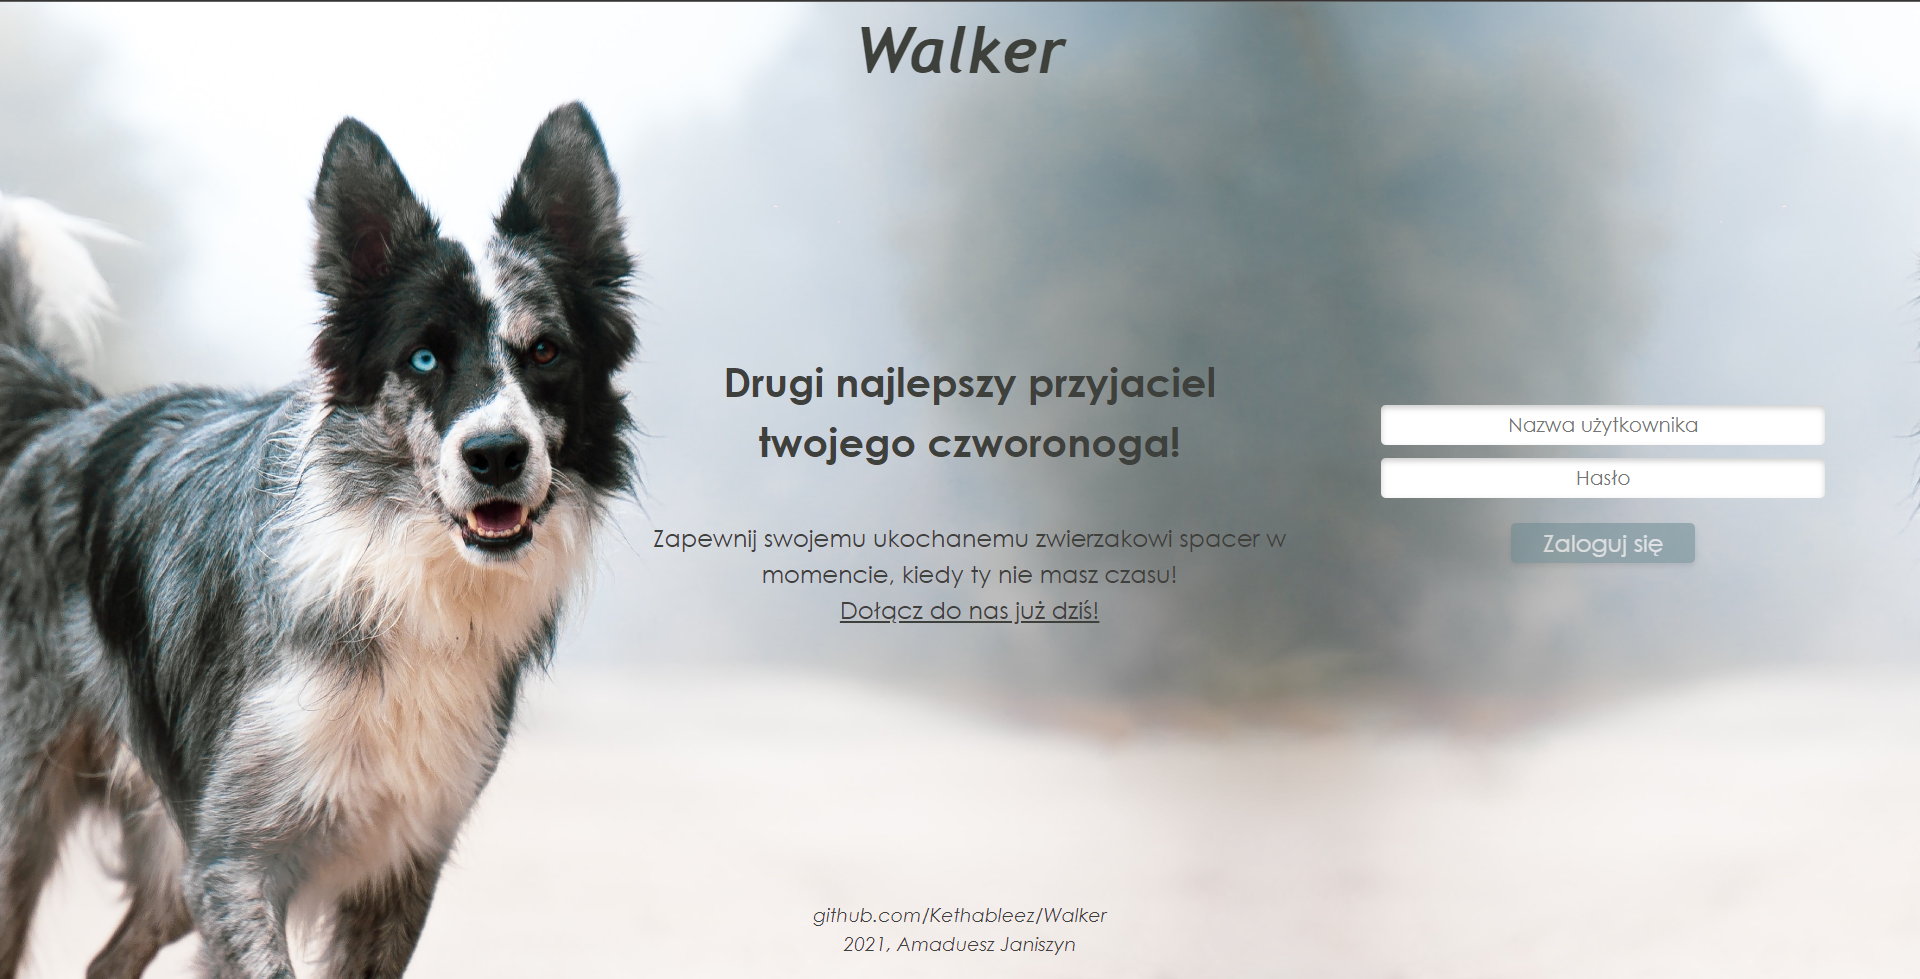
\includegraphics[width=1\linewidth]{rysunki/walker-1.PNG}
  \caption{Strona startowa}
  \label{fig:walker-landing-page}
\end{figure}


\begin{figure}[H]
  \centering
  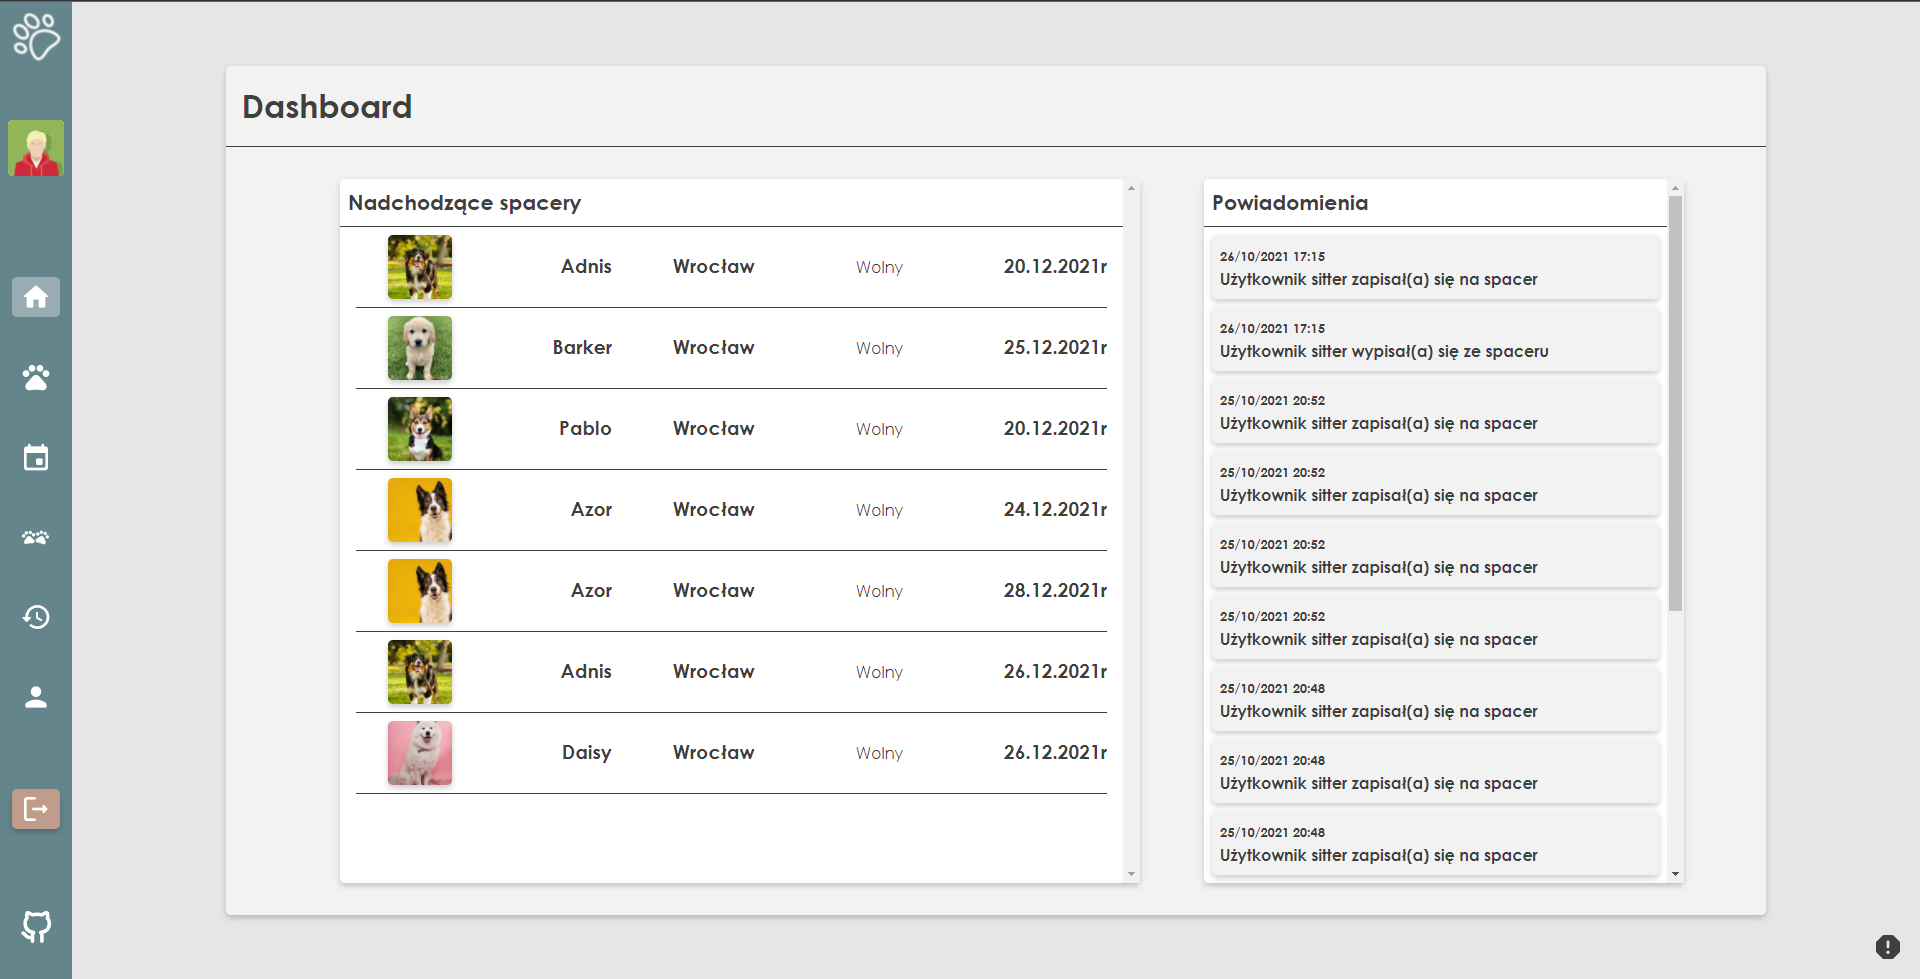
\includegraphics[width=1\linewidth]{rysunki/walker-2.PNG}
  \caption{Dashboard}
  \label{fig:walker-dashboard}
\end{figure}


\begin{figure}[H]
  \centering
  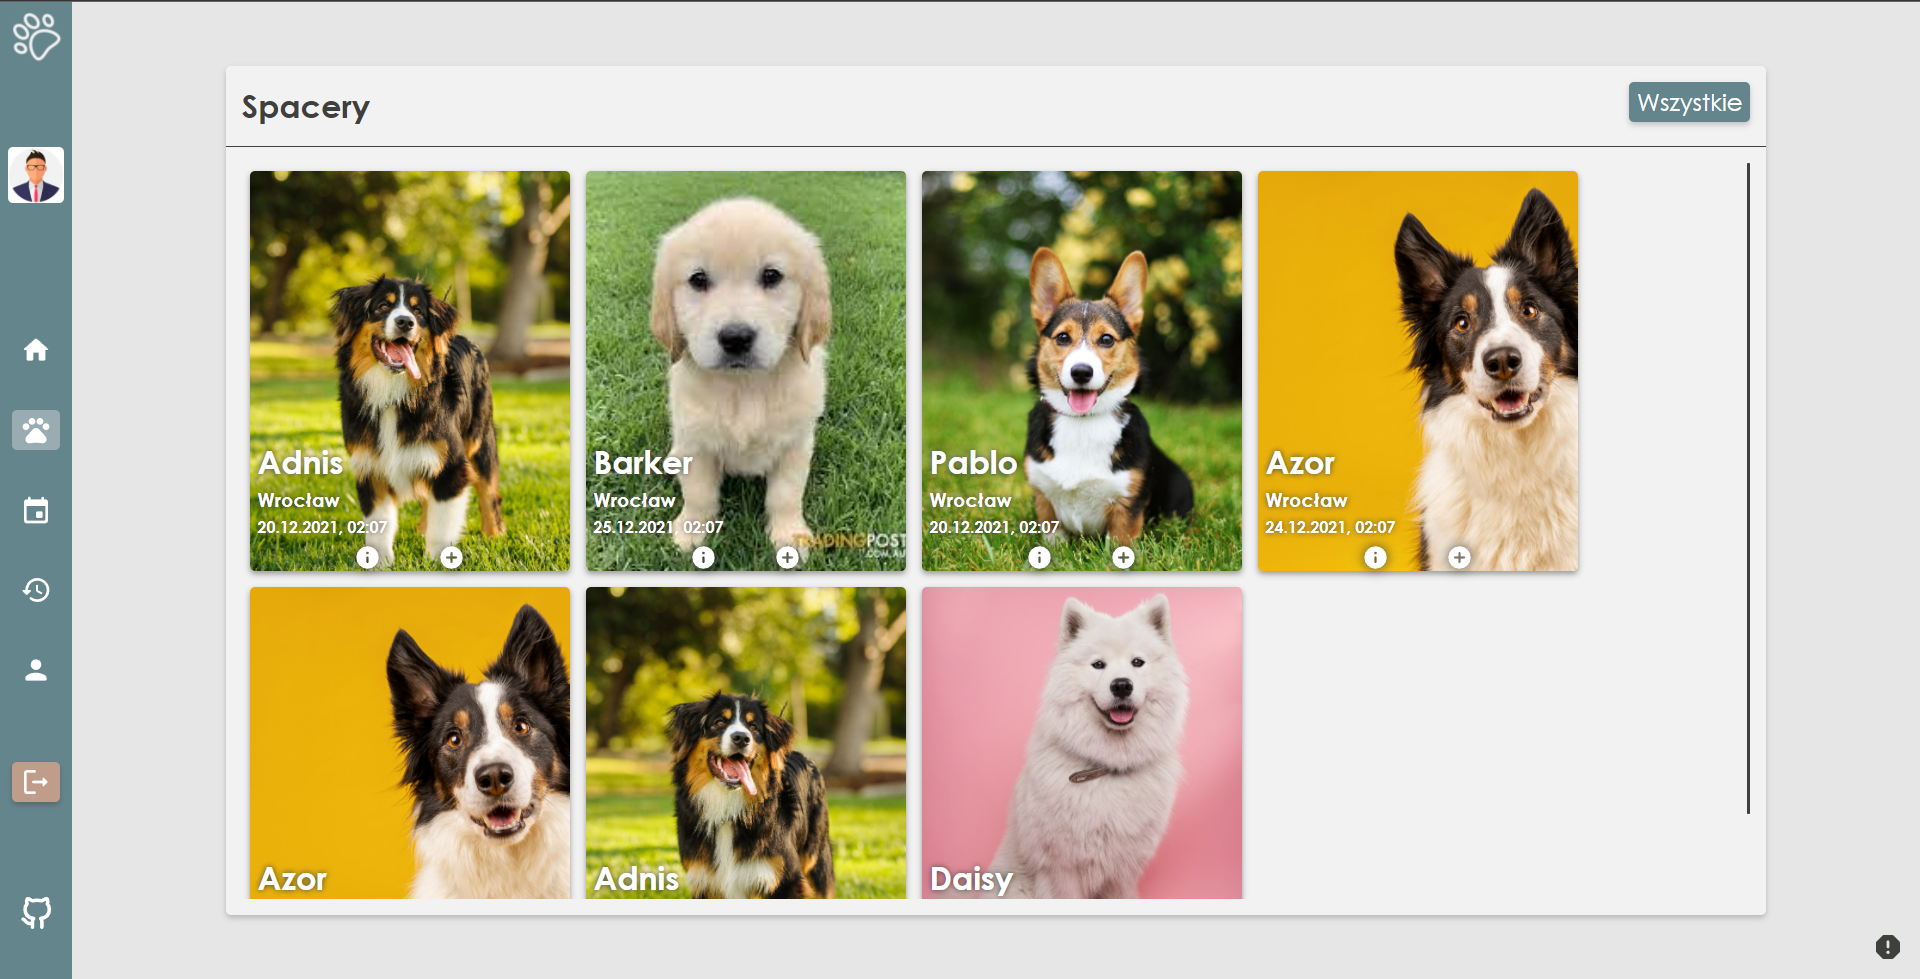
\includegraphics[width=1\linewidth]{rysunki/walker-3.PNG}
  \caption{Lista spacerów}
  \label{fig:walker-walk-list}
\end{figure}


\begin{figure}[H]
  \centering
  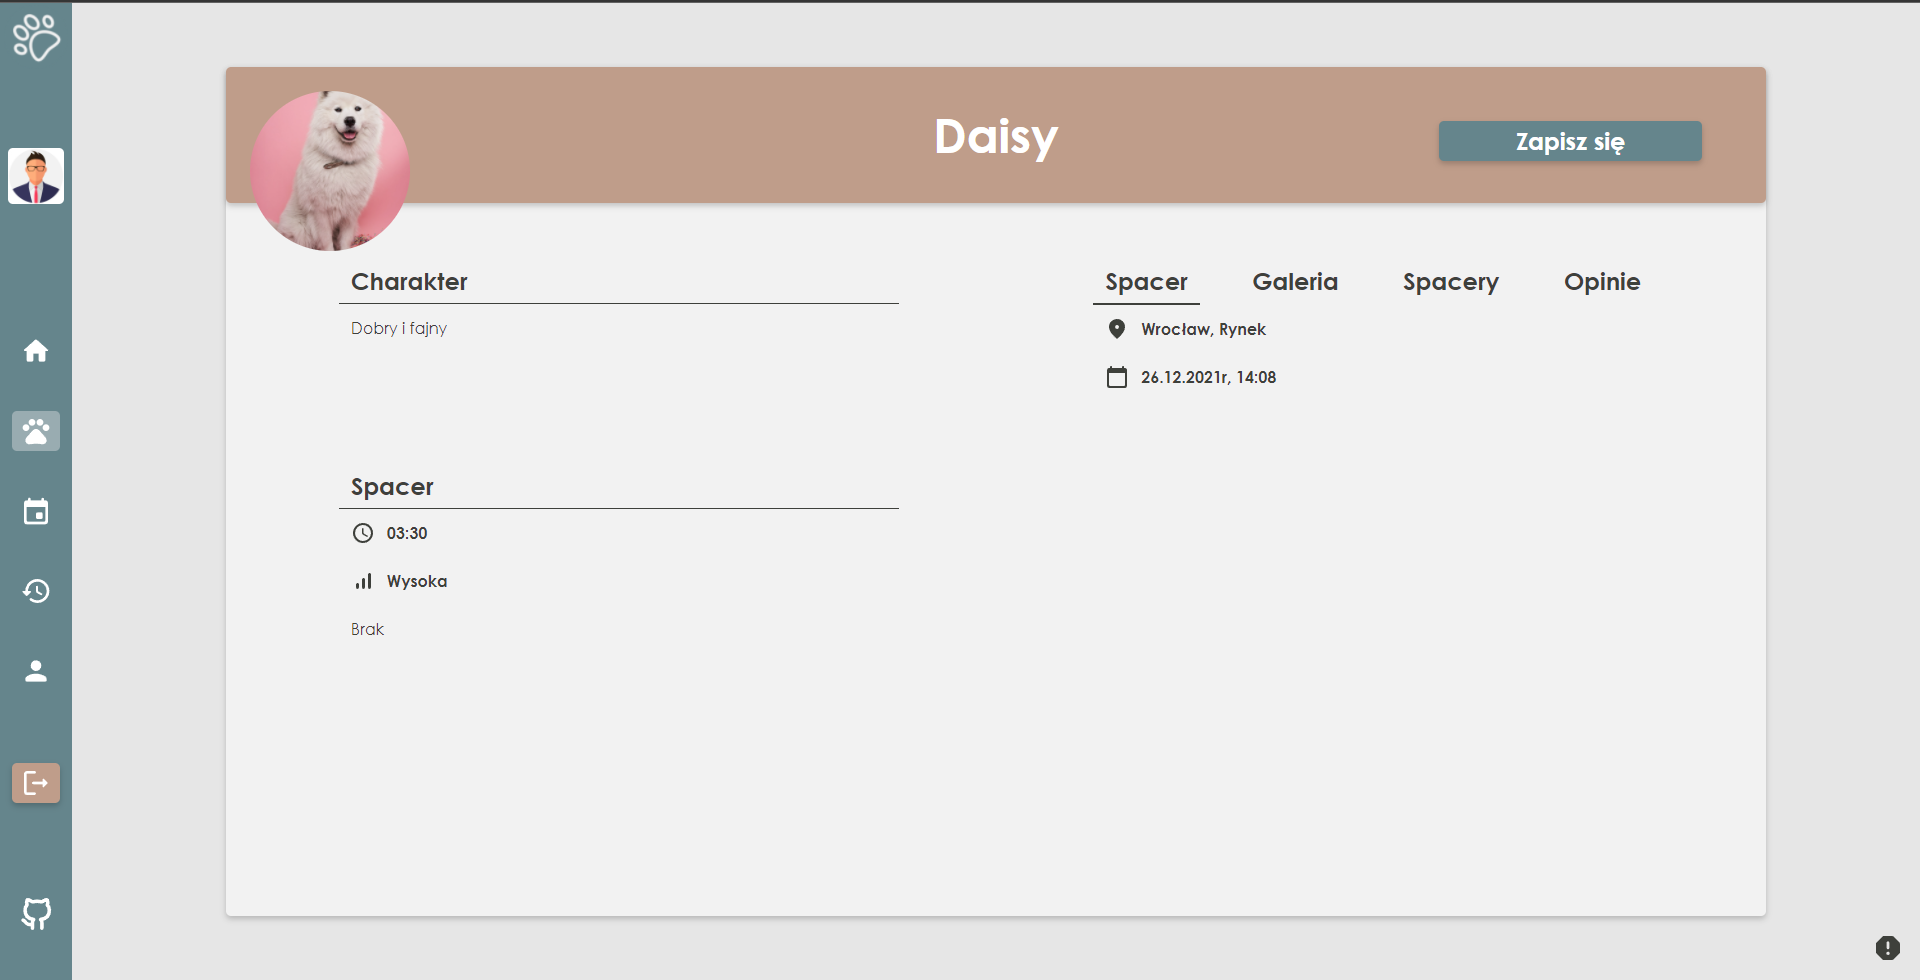
\includegraphics[width=1\linewidth]{rysunki/walker-4.PNG}
  \caption{Profil psa}
  \label{fig:walker-dog-profile}
\end{figure}


\begin{figure}[H]
  \centering
  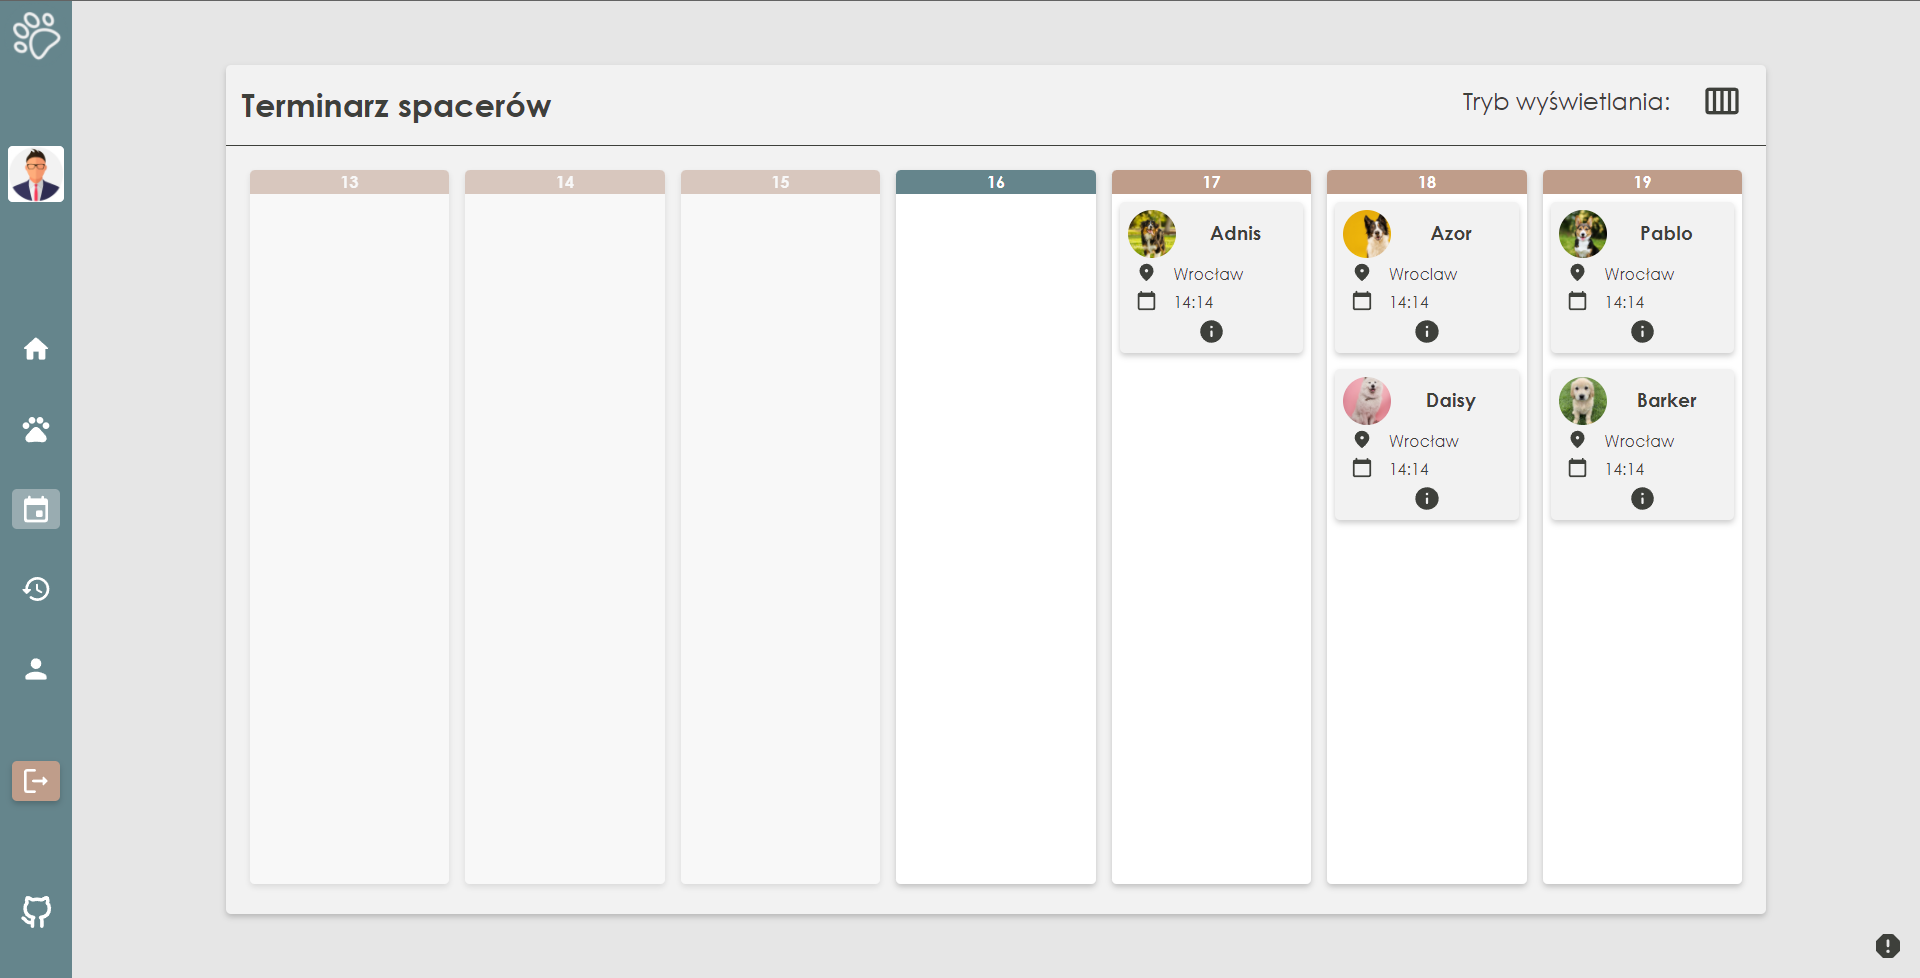
\includegraphics[width=1\linewidth]{rysunki/walker-5.PNG}
  \caption{Kalendarz -- widok tygodnia}
  \label{fig:walker-calendar-week}
\end{figure}


\begin{figure}[H]
  \centering
  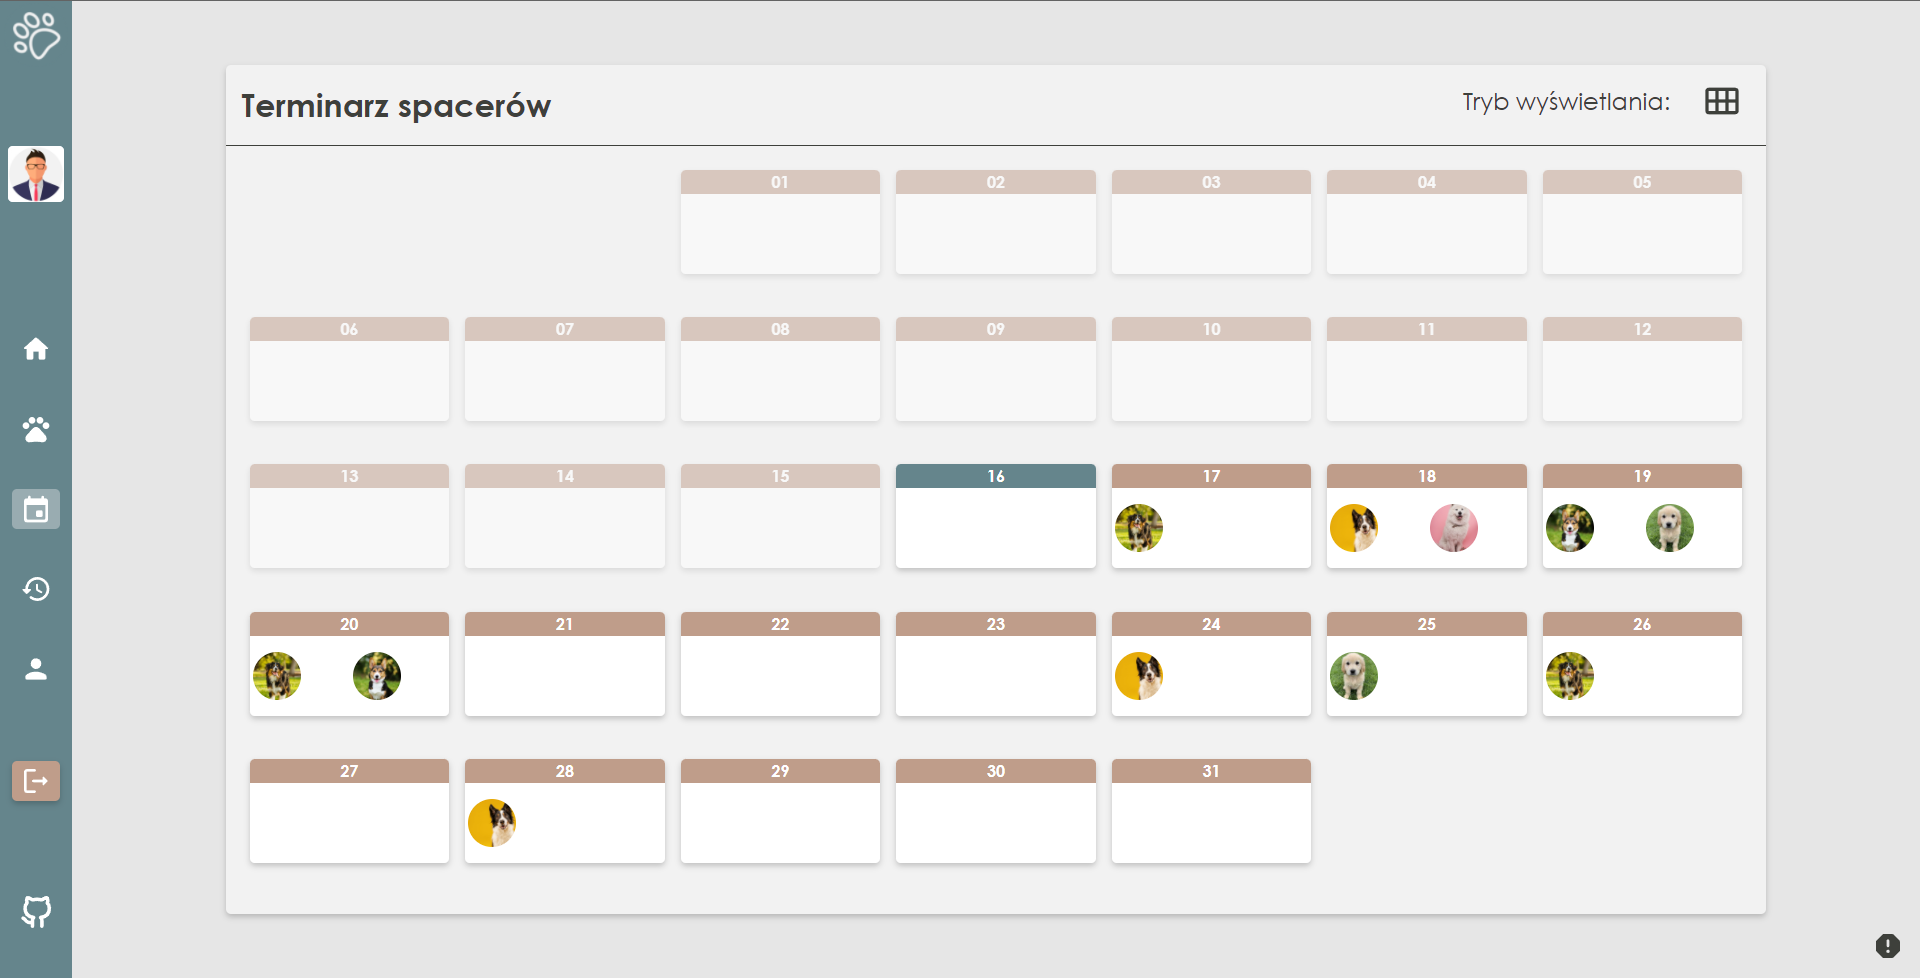
\includegraphics[width=1\linewidth]{rysunki/walker-7.PNG}
  \caption{Kalendarz -- widok miesiąca}
  \label{fig:walker-calendar-month}
\end{figure}


\subsection{JWT -- Autoryzacja i autentykacja}
Proces implementacji autoryzacji użytkowników przez mechanizm JWT rozpoczęto od stworznia metody odpowiedzialnej za wysyłanie formularza logowania do backendu:
\begin{lstlisting}
  loginUser(credentials: any): Observable<any> {
    const url = this.setting.getAuthUrl('loginUser');

    return this.http.post(url, {
      username: credentials.username,
      password: credentials.password
    }, httpOptions);
  }
\end{lstlisting}

Metoda zostaje wywołana w momencie naciśnięcia przycisku \textit{Zaloguj się}.
\begin{lstlisting}
  loginUser(): void {
    this.authService.loginUser(this.loginForm.value).subscribe(
      data => {
        this.saveAuthTokenAfterLogin(data.token);
      }
    );
  }
\end{lstlisting}

Po pomyślnym zalogowaniu, do aplikacji dostępowej zostaje wysłany token autoryzacyjny, który następnie przy pomocy klasy \textit{TokenStorageService} zapisuje go w sesji przeglądarki.
\begin{lstlisting}
  const TOKEN_KEY = 'auth-token';

  public saveToken(token: string): void {
    window.sessionStorage.removeItem(TOKEN_KEY);
    window.sessionStorage.setItem(TOKEN_KEY, token);
  }
\end{lstlisting}

Zapisany token zostaje następnie wstrzykiwany do każdego zapytania wysyłanego do backendu przez zalogowanego użytkownika. Odpowiada za to klasa \textit{AuthInterceptor} oraz metoda \textit{intercept}:
\begin{lstlisting}
  intercept(req: HttpRequest<any>, next: HttpHandler): 
                                        Observable<HttpEvent<any>> {
    let authReq = req;
    const token = this.token.getToken();
    if (token != null) {
      authReq = req.clone({ 
        headers: req.headers.set(TOKEN_HEADER_KEY, 'Bearer ' + token) 
        });
    }
    return next.handle(authReq);
  }
\end{lstlisting}

\subsection{Biblioteki i moduły}
Wykorzystane biblioteki oraz moduły wspomogły proces implementacyjny oraz udostępniły szereg funkcjonalności, bez których nie byłoby możliwe stworzenie rozbudowanej aplikacji dostępowej.
\begin{lstlisting}
  imports: [
    BrowserModule,
    AppRoutingModule,
    ReactiveFormsModule,
    HttpClientModule,
    NgbModule
  ]
\end{lstlisting}

\subsubsection{AppRoutingModule}
\begin{figure}[H]
  \centering
  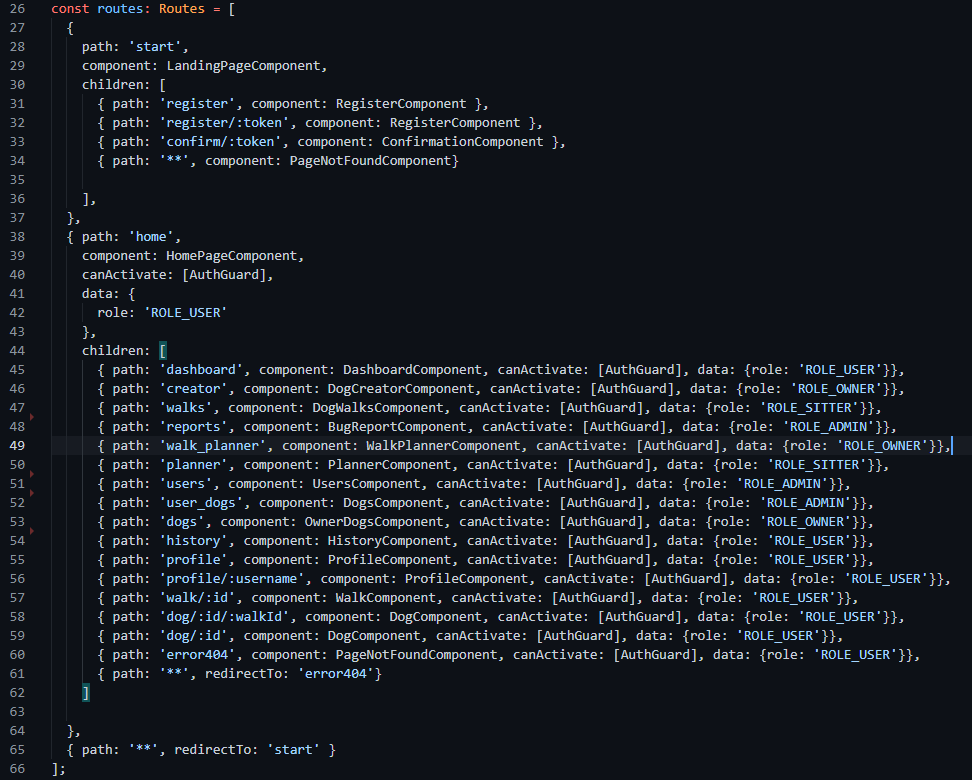
\includegraphics[width=0.7\linewidth]{rysunki/routes.PNG}
  \caption{Implementacja nawigacji}
  \label{fig:walker-routes}
\end{figure}
Dzięki temu modułowi, możliwe było zadeklarowanie ścieżek aplikacji, z uwzględnieniem poszczególnych komponentów oraz zabezpieczenie przed użytkownikami, którzy nie posiadają odpowiedniej roli.

\subsubsection{ReactiveFormsModule}
\begin{lstlisting}
    dogForm = this.builder.group({
      name: ['', Validators.required],
      dogBreed: ['', Validators.required],
      dogPhoto: ['', Validators.required],
      dogType: ['', Validators.required],
      characteristic: ['', 
          [Validators.required, 
          Validators.maxLength(255)]],
      walkDuration: ['', 
          [Validators.required, 
          Validators.pattern('[0-9]{2}:[0-9]{2}')]],
      walkIntensity: ['', Validators.required],
      walkDescription: ['', 
          [Validators.required, 
          Validators.maxLength(255)]],
  });
\end{lstlisting}

\subsubsection{HttpClientModule}
\begin{lstlisting}
  getOwnerData(username?: string) {
    const url = this.setting.getOwnerUrl(
      'getData', 
      {username: username}
      );

    return this.http.get<OwnerData>(url);
  }
\end{lstlisting}

\subsubsection{NgbModule}
\begin{lstlisting}
  <ngb-rating 
  [max]="5"
  formControlName="rating">
  </ngb-rating>
\end{lstlisting}

\subsubsection{RxJS}
\begin{lstlisting}
  this.users = this.users.pipe(
    map((users: UserWithInfo[]) => {
      return removeById(users, user.id);
    })
  );
\end{lstlisting}
